\documentclass[11pt,a4paper]{article}
\usepackage[no-math]{fontspec}
\usepackage{mathptmx}
\setmainfont{TeX Gyre Termes}
\usepackage{polyglossia}
\setdefaultlanguage[variant=british]{english}
\usepackage{amsmath,amssymb,amsthm,bm}
\usepackage{booktabs,array,threeparttable,adjustbox}
\usepackage{graphicx}
\usepackage[labelfont=bf,labelsep=space,font=small,justification=centering]{caption}
\captionsetup[figure]{name=Fig.}\captionsetup[table]{name=Table}
\usepackage{lineno}
\usepackage[a4paper,margin=2.6cm]{geometry}
\usepackage{setspace}
\usepackage[authoryear,round]{natbib}
\bibpunct{(}{)}{;}{a}{}{,}
\usepackage{microtype}
\usepackage{enumitem}
\usepackage[hidelinks]{hyperref}
\usepackage{titlesec}
\usepackage[section]{placeins}
\titleformat{\section}{\normalfont\large\bfseries}{\thesection}{0.6em}{}
\titleformat{\subsection}{\normalfont\bfseries\itshape}{\thesubsection}{0.5em}{}
\titlespacing*{\section}{0pt}{2.2ex plus 1ex}{1.2ex}
\titlespacing*{\subsection}{0pt}{1.8ex plus 0.8ex}{0.8ex}
\setstretch{1.5}
\setlength{\parskip}{0pt}
\setlength{\parindent}{1.4em}
\setlength{\emergencystretch}{2em}
\renewcommand{\arraystretch}{1.08}
\setlist{nosep,leftmargin=1.6em}
\renewcommand{\floatpagefraction}{0.75}
\renewcommand{\topfraction}{0.85}
\renewcommand{\textfraction}{0.12}
\newtheorem{proposicion}{Proposition}
\newcommand{\cenFullB}{0.13}
\newcommand{\cenFullSe}{0.10}
\newcommand{\cenFullF}{29.0}
\newcommand{\cenFullAR}{[$-$0.08, 0.35]}
\newcommand{\cenFullWCR}{[$-$0.15, 0.36]}
\newcommand{\cenFullRI}{[0.02, 0.26]}
\newcommand{\cenFullRIcont}{$(-\infty,\infty)$}
\newcommand{\cenFullAKM}{[$-$0.65, 0.44]}
\newcommand{\cenFullRIp}{0.038}
\newcommand{\origFullB}{0.30}
\newcommand{\origFullSe}{0.12}
\newcommand{\origFullAR}{[0.09, 0.58]}
\newcommand{\origFullAKM}{[$-$0.08, 0.90]}
\newcommand{\origFullF}{32.2}
\newcommand{\origFullRI}{[0.15, 0.44]}
\newcommand{\origFullWCR}{[0.03, 0.59]}
\newcommand{\sizeFullB}{0.01}
\newcommand{\sizeFullAR}{[$-$0.23, 0.30]}
\newcommand{\minFullB}{0.55}
\newcommand{\minFullAR}{[0.33, 0.87]}
\newcommand{\cenArrB}{0.24}
\newcommand{\cenArrSe}{0.11}
\newcommand{\cenArrF}{14.4}
\newcommand{\cenArrAR}{[0.07, 0.59]}
\newcommand{\cenArrWCR}{[0.06, 0.59]}
\newcommand{\cenArrRI}{[0.15, 0.34]}
\newcommand{\cenArrRIcont}{[$-\infty$, 1.00]}
\newcommand{\cenArrAKM}{[$-$0.56, 0.82]}
\newcommand{\cenArrRIp}{0.003}
\newcommand{\origArrB}{0.45}
\newcommand{\origArrSe}{0.16}
\newcommand{\origArrAR}{[0.21, 0.99]}
\newcommand{\origArrAKM}{[0.13, $\infty$]}
\newcommand{\origArrF}{14.6}
\newcommand{\origArrRI}{[0.28, 0.62]}
\newcommand{\origArrWCR}{[0.19, 0.96]}
\newcommand{\sizeArrB}{0.13}
\newcommand{\sizeArrAR}{[$-$0.06, 0.52]}
\newcommand{\minArrB}{0.62}
\newcommand{\minArrAR}{[0.38, 1.05]}
\newcommand{\cenFullRB}{0.14}
\newcommand{\cenFullRSe}{0.09}
\newcommand{\cenFullRF}{36.2}
\newcommand{\cenFullRAR}{[$-$0.02, 0.33]}
\newcommand{\cenFullRWCR}{[$-$0.07, 0.34]}
\newcommand{\cenFullRRI}{[0.07, 0.23]}
\newcommand{\cenFullRRIcont}{$(-\infty,\infty)$}
\newcommand{\cenFullRAKM}{[$-$0.65, 0.38]}
\newcommand{\cenFullRRIp}{0.011}
\newcommand{\origFullRB}{0.30}
\newcommand{\origFullRSe}{0.10}
\newcommand{\origFullRAR}{[0.12, 0.54]}
\newcommand{\origFullRAKM}{[$-$0.02, 0.76]}
\newcommand{\origFullRF}{36.4}
\newcommand{\origFullRRI}{[0.20, 0.43]}
\newcommand{\origFullRWCR}{[0.07, 0.54]}
\newcommand{\sizeFullRB}{0.03}
\newcommand{\sizeFullRAR}{[$-$0.19, 0.27]}
\newcommand{\minFullRB}{0.50}
\newcommand{\minFullRAR}{[0.31, 0.84]}
\newcommand{\cenArrRB}{0.20}
\newcommand{\cenArrRSe}{0.09}
\newcommand{\cenArrRF}{17.3}
\newcommand{\cenArrRAR}{[0.06, 0.47]}
\newcommand{\cenArrRWCR}{[0.03, 0.49]}
\newcommand{\cenArrRRI}{[0.14, 0.26]}
\newcommand{\cenArrRRIcont}{$(-\infty,\infty)$}
\newcommand{\cenArrRAKM}{[$-$0.94, 0.48]}
\newcommand{\cenArrRRIp}{0.001}
\newcommand{\origArrRB}{0.39}
\newcommand{\origArrRSe}{0.14}
\newcommand{\origArrRAR}{[0.17, 0.83]}
\newcommand{\origArrRAKM}{[0.04, $\infty$]}
\newcommand{\origArrRF}{15.1}
\newcommand{\origArrRRI}{[0.27, 0.55]}
\newcommand{\origArrRWCR}{[0.14, 0.87]}
\newcommand{\sizeArrRB}{0.12}
\newcommand{\sizeArrRAR}{[$-$0.07, 0.43]}
\newcommand{\minArrRB}{0.51}
\newcommand{\minArrRAR}{[0.34, 0.84]}
\newcommand{\cenFullUB}{0.01}
\newcommand{\cenFullUSe}{0.16}
\newcommand{\cenFullUF}{15.7}
\newcommand{\cenFullUAR}{[$-$0.37, 0.34]}
\newcommand{\cenFullUWCR}{[$-$0.42, 0.37]}
\newcommand{\cenFullURI}{[$-$0.16, 0.38]}
\newcommand{\cenFullURIcont}{$(-\infty,\infty)$}
\newcommand{\cenFullUAKM}{[$-$1.26, 0.75]}
\newcommand{\cenFullURIp}{0.381}
\newcommand{\origFullUB}{0.21}
\newcommand{\origFullUSe}{0.15}
\newcommand{\origFullUAR}{[$-$0.11, 0.57]}
\newcommand{\origFullUAKM}{[$-$0.63, 1.03]}
\newcommand{\origFullUF}{14.5}
\newcommand{\origFullURI}{[0.02, 0.60]}
\newcommand{\origFullUWCR}{[$-$0.18, 0.60]}
\newcommand{\sizeFullUB}{$-$0.02}
\newcommand{\sizeFullUAR}{[$-$0.48, 0.39]}
\newcommand{\minFullUB}{0.35}
\newcommand{\minFullUAR}{[0.08, 0.83]}
\newcommand{\cenArrUB}{0.19}
\newcommand{\cenArrUSe}{0.20}
\newcommand{\cenArrUF}{6.1}
\newcommand{\cenArrUAR}{[$-$0.15, 1.41]}
\newcommand{\cenArrUWCR}{[$-$0.15, 1.43]}
\newcommand{\cenArrURI}{[0.07, 0.60]}
\newcommand{\cenArrURIcont}{$(-\infty,\infty)$}
\newcommand{\cenArrUAKM}{$(-\infty,\infty)$}
\newcommand{\cenArrURIp}{0.021}
\newcommand{\origArrUB}{0.57}
\newcommand{\origArrUSe}{0.30}
\newcommand{\origArrUAR}{[0.17, 3.65]}
\newcommand{\origArrUAKM}{$(-\infty,\infty)$}
\newcommand{\origArrUF}{5.3}
\newcommand{\origArrURI}{[0.41, 1.31]}
\newcommand{\origArrUWCR}{[0.14, 3.51]}
\newcommand{\sizeArrUB}{0.19}
\newcommand{\sizeArrUAR}{[$-$0.24, 1.70]}
\newcommand{\minArrUB}{0.66}
\newcommand{\minArrUAR}{[0.32, $\infty$]}
\newcommand{\effN}{15.8}
\newcommand{\corrAll}{0.71}
\newcommand{\autoc}{0.64}
\newcommand{\corrAme}{0.85}
\newcommand{\corrEur}{0.68}
\newcommand{\Jstat}{137.4}
\newcommand{\limlB}{0.17}
\newcommand{\limlSe}{0.09}
\newcommand{\rotRom}{0.31}
\newcommand{\rotCol}{0.21}
\newcommand{\gRom}{$-$2.33}
\newcommand{\rotNeg}{$-$0.17}
\newcommand{\balConstr}{$-$0.87}
\newcommand{\balConstrP}{0.001}
\newcommand{\balConstrW}{$-$1.21}
\newcommand{\balConstrWP}{0.008}
\newcommand{\balRent}{0.59}
\newcommand{\balRentP}{0.018}
\newcommand{\balTert}{0.51}
\newcommand{\balTertP}{0.049}
\newcommand{\natIV}{0.23}
\newcommand{\bhjEq}{0.226}
\newcommand{\bhjYfe}{0.234}
\newcommand{\akmOrig}{[$-$0.07, 0.96]}
\newcommand{\akmOY}{[0.05, 0.48]}
\newcommand{\preW}{$-$0.085}
\newcommand{\preWse}{0.046}
\newcommand{\preWp}{0.075}
\newcommand{\rfLDW}{0.102}
\newcommand{\rfLDWse}{0.043}
\newcommand{\natPreOrig}{0.41}
\newcommand{\natPreOrigP}{0.004}
\newcommand{\natPreCen}{$-$0.011}
\newcommand{\natPreCenP}{0.89}
\newcommand{\permP}{0.35}
\newcommand{\boomCorr}{0.74}
\newcommand{\lpFcov}{2.8}
\newcommand{\lpFmin}{6.8}
\newcommand{\wOut}{$-$0.01}
\newcommand{\wOutSe}{0.26}
\newcommand{\wIn}{0.45}
\newcommand{\wInAR}{[0.21, 0.99]}
\newcommand{\wTwoZeroTwoFour}{0.31}
\newcommand{\wTwoZeroTwoFourAR}{[0.05, 2.28]}
\newcommand{\wTwoZeroTwoFourold}{$-$0.46}
\newcommand{\calB}{0.05}
\newcommand{\cenB}{0.31}
\newcommand{\swFOne}{8.7}
\newcommand{\epBW}{0.64}
\newcommand{\epSeW}{0.20}
\newcommand{\epFW}{9.4}
\newcommand{\epARW}{[0.22, 1.27]}
\newcommand{\epWCRW}{[0.04, 1.80]}
\newcommand{\epBR}{0.68}
\newcommand{\epSeR}{0.18}
\newcommand{\epFR}{9.4}
\newcommand{\epARR}{[0.31, 1.25]}
\newcommand{\epWCRR}{[0.10, 1.92]}
\newcommand{\epBU}{0.27}
\newcommand{\epSeU}{0.24}
\newcommand{\epFU}{4.3}
\newcommand{\epARU}{[$-$1.68, 1.27]}
\newcommand{\epWCRU}{$(-\infty,\infty)$}
\newcommand{\crowdC}{0.45}
\newcommand{\crowdCse}{0.15}
\newcommand{\popC}{0.70}
\newcommand{\popCse}{0.24}
\newcommand{\natC}{$-$0.30}
\newcommand{\vacC}{1.00}
\newcommand{\vacCse}{0.50}
\newcommand{\newC}{$-$0.74}
\newcommand{\newCse}{0.55}
\newcommand{\dlnsC}{0.46}
\newcommand{\dlnsCse}{0.15}
\newcommand{\shareC}{0.64}
\newcommand{\shareCfi}{[0.34, 1.19]}
\newcommand{\shareCbo}{[$-$0.53, 1.73]}
\newcommand{\shareA}{0.56}
\newcommand{\shareAfi}{[0.23, 1.02]}
\newcommand{\shareAU}{0.37}
\newcommand{\shareCU}{0.60}
\newcommand{\shareCUfi}{[0.04, 7.95]}
\newcommand{\shareMin}{3.70}
\newcommand{\compC}{$-$0.08}
\newcommand{\withinC}{0.54}
\newcommand{\ratioP}{0.96}
\newcommand{\ratioPse}{0.12}
\newcommand{\stockP}{$-$0.24}
\newcommand{\stockPse}{0.16}
\newcommand{\panelF}{4.9}
\newcommand{\outES}{$-$0.05}
\newcommand{\outESse}{0.19}
\newcommand{\outESF}{3.5}
\newcommand{\kapEur}{1.10}
\newcommand{\kapAfr}{0.64}
\newcommand{\kapAme}{0.96}
\newcommand{\kapAsi}{0.68}
\newcommand{\shareArr}{7.5}
\newcommand{\shareArrLo}{2.2}
\newcommand{\shareArrHi}{18.6}
\newcommand{\shareFullHi}{11.0}
\newcommand{\shareFull}{4.1}
\newcommand{\shareEp}{20.1}
\newcommand{\shareOrig}{9.6}
\newcommand{\turnover}{0.31}
\newcommand{\passT}{0.034}
\newcommand{\passLOne}{0.039}
\newcommand{\passLTwo}{0.036}
\newcommand{\catF}{4.2}
\newcommand{\catN}{123}
\newcommand{\altF}{0.11}
\newcommand{\spContig}{0.06}
\newcommand{\spContigSe}{0.07}

\newcommand{\E}{\mathbb{E}}

\title{\bfseries Immigration, Rents and Housing Occupancy in Spain}
\author{Víctor M. Fernández-Aguilera\\[4pt]
{\small University of Almería, Almería, Spain}\\
{\small Corresponding author. E-mail: vfa084@ual.es}}
\date{}

\begin{document}
\maketitle

\begin{abstract}\noindent
Spain's foreign-born population grew by more than three million between 2015 and 2025 while the official rent index rose by about a fifth. Using tax-based rent indices for 699 municipalities, population registers by country of birth, census tracts and the cadastre, this paper studies how local rents and the use of the housing stock responded to immigrant inflows predicted from the 2003 settlement of 33 origin groups. Origin shocks are few in effective number and strongly correlated, so the design is assessed with shock-level diagnostics, falsification tests and inference robust to weak instruments and to exposure-induced correlation. Additional population was housed within the existing stock: registered population per cadastral dwelling rose with inflows, the stock did not respond detectably in the short run, and persons per primary dwelling rose between the 2011 and 2021 censuses. Within provinces, in the arrival years 2015--2024 an inflow equal to 1\,\% of the population is associated with a rise of about \cenArrB\,\% in the average rent of declared contracts in force (95\,\% Anderson-Rubin set \cenArrAR), once municipalities may follow trends that differ by predetermined demographic and economic structure. This estimate is smaller than in specifications with fewer controls and is not robust to exposure-robust inference that clusters shocks by origin or to identification from within-continent variation. A sharper episode, the 2016 Schengen visa waivers for Colombia and Peru, yields a larger relative effect in large municipalities. Under explicit assumptions, immigration accounts for a minority of national rent-index growth in 2015--2024.

\medskip\noindent\textbf{Keywords} Immigration $\cdot$ Housing rents $\cdot$ Housing occupancy $\cdot$ Shift-share instruments $\cdot$ Spain\\
\textbf{JEL Classification} J61 $\cdot$ R21 $\cdot$ R31
\end{abstract}
\clearpage
\linenumbers

\section{Introduction}\label{sec:intro}

Spain's foreign-born population fell from 6.68 to 6.16 million between 2011 and 2015, as emigration followed the financial crisis, and has since grown to 9.46 million, 19.3\,\% of residents on 1 January 2025. Over the same period the official rent index rose by more than 20\,\%, and housing became a main economic concern of young households and of those who arrive. The coincidence has made immigration a leading explanation for rising rents in public debate. Credible estimates with recent Spanish data are scarce, and so is an account of how newcomers were housed.

How newcomers are housed matters for the size of any price effect. A person who moves into a room in a shared flat or into a relative's household adds population but not demand for an additional dwelling; if vacant or second homes are brought back into use, the occupied stock grows without construction; and if residents move to another municipality within the same market, the pressure of a localised inflow spreads. Each margin dampens the local rent response. Measuring rents without measuring how intensively the stock is used gives an incomplete picture of the adjustment.

The paper combines the rental housing price index (IPVA) that the Spanish Statistical Office (INE) builds from personal income tax returns, available for 699 municipalities with more than 10,000 inhabitants between 2011 and 2024, with the municipal population register and the annual population census by country of birth for 33 origins, tract-level indicators from the 2011 and 2021 censuses, the cadastral housing stock, the firm directory, the deposit register of new rental contracts in Catalonia and Eurostat migration statistics. The empirical strategy compares municipalities within the same province and year and instruments immigrant inflows with the prediction obtained by combining each origin's 2003 settlement pattern with its subsequent national growth.

The first contribution is a careful evaluation of what this design can identify in the Spanish case. The origin shocks are few in effective number (\effN) and strongly correlated with each other (mean pairwise correlation \corrAll), and identification relies heavily on two origins, Romania, whose national stock fell continuously after 2012, and Colombia. Predicted inflows are correlated with predetermined municipal characteristics, and national origin growth is correlated with the construction intensity of the municipalities exposed to each origin. The paper therefore reports shock-level diagnostics, falsification tests with genuine pre-periods, and four layers of inference: Anderson-Rubin sets with province clusters and with a restricted wild bootstrap, randomisation inference with recentred instruments under explicitly stated assignment strata \citep{borusyak2023}, and the null-imposed exposure-robust test of \citet{adao2019}.

The second contribution concerns rents, and the estimates call for caution. In the original specification of this paper, which controlled for 2015 income per person and three other characteristics, the within-province elasticity was \origFullB{} over 2012--2024. That control is measured inside the sample period, and the estimate is sensitive to how municipal trends are modelled: allowing trends to differ by predetermined 2011 education and age structure and by 2012 economic structure, the central specification of this revision, gives \cenFullB{} over 2012--2024 (Anderson-Rubin set \cenFullAR) and \cenArrB{} in the arrival years 2015--2024 (\cenArrAR). The response is absent in 2012--2014, when the foreign-born population fell. The arrival-period estimate excludes zero under province-clustered and wild-bootstrap inference and under randomisation across all origins, but not under exposure-robust inference that clusters shocks by origin (\cenArrAKM) or when identification is restricted to the composition of immigration within continents. A sharper source of variation, the 2016 Schengen visa waivers for Colombia and Peru, which compares municipalities with similar Latin American exposure and shows no pre-trends in rents, yields a larger relative effect in population-weighted estimates, \epBW{} per percentage point of inflow (wild-bootstrap Anderson-Rubin set \epWCRW), and an imprecise one without weights.

The third contribution documents the quantity side. Between the 2011 and 2021 censuses, each additional immigrant is associated with \crowdC{} more persons housed through higher occupancy of primary dwellings, while the cadastral stock did not grow faster where more immigrants arrived. The share of net population growth absorbed by higher occupancy is imprecisely estimated (\shareC, Fieller interval \shareCfi), and, at the level of continental groups, the change is not explained by the composition of residents. Higher occupancy is not the same as overcrowding, and the paper does not observe rooms or welfare; it documents that the existing stock was used more intensively, not that living conditions worsened.

These findings qualify the existing evidence for Spain, which mostly concerns sale prices in the 2000s \citep{gonzalez2013,sanchis2023}, and the international evidence that rent effects are smaller at finer spatial scales \citep{saiz2011,accetturo2014}. Methodologically, the paper shows in a policy-relevant application how conclusions from a shift-share design depend on the control for predetermined trends, on the separation of inflow and outflow years, and on the assignment process assumed for the shocks.

Section~\ref{sec:lit} reviews the evidence and section~\ref{sec:model} presents a conceptual framework. Section~\ref{sec:data} describes the institutional setting, data and measurement, and section~\ref{sec:empirics} the empirical design and its diagnostics. Section~\ref{sec:rents} reports the effects on rents and section~\ref{sec:validity} the validity checks and the visa-waiver episode. Section~\ref{sec:margins} studies the margins of adjustment, section~\ref{sec:magnitude} the aggregate magnitudes, section~\ref{sec:discussion} discusses interpretation and policy, and section~\ref{sec:conclusion} concludes.

\section{Previous evidence}\label{sec:lit}

\subsection{Immigration, prices and rents}

The classic references are \citet{saiz2003}, who documents a rise in Miami rents after the Mariel boatlift, and \citet{saiz2007}, who estimates for US metropolitan areas that an inflow equal to 1\,\% of the population raises rents and prices by about 1\,\%. European estimates tend to be larger for sale prices: \citet{degen2017} find 2.7\,\% for Swiss single-family homes and \citet{unal2026}, for 382 German districts, up to 3\,\% for flat prices and about 1\,\% for flat rents; \citet{akbari2012} find positive effects in Canada. The sign changes when comparisons are made at fine scales or when residents move. \citet{sa2015} obtains negative effects in the United Kingdom driven by the outflow of high-income residents, \citet{saiz2011} document slower price growth in US neighbourhoods where immigrants settle and \citet{accetturo2014} show for Italy that the effect is positive across cities and negative across neighbourhoods. In sudden-arrival episodes, \citet{balkan2018} find rent increases after the arrival of Syrian refugees in Turkey, an episode whose effects on employment and consumer prices are analysed by \citet{tumen2016} and \citet{balkan2016}, and \citet{mussa2017} stress spatial spillovers.

For Spain, \citet{gonzalez2013} attribute a substantial part of the price and construction boom of 2000--2010 to immigration, and \citet{sanchis2023} estimates with 2001--2012 data that one percentage point of immigration raises sale prices by 3.3\,\%, a figure that depends on native relocation. \citet{fernandez2019} use geocoded addresses to show that immigrant inflows between 1998 and 2008 caused a mild outflow of natives from dense, established neighbourhoods, offset by suburban development. Work at the Banco de España describes the expansion of renting and the rising burden on households \citep{lopez2019,khametshin2024} and lists demographic growth among the recent drivers of demand \citep{bde2024,lajer2024}. \citet{garcia2020} estimate the effect of short-term rentals in Barcelona and \citet{monras2023} that of rent controls in Catalonia. None of these studies covers the post-2015 migration wave with tax-based rents or measures the margins through which newcomers are housed.

\subsection{Occupancy, mobility, supply and shift-share designs}

\citet{myers1996} and \citet{myerslee1996} document high overcrowding among recent immigrant cohorts that declines with length of residence. The response of natives has been studied mostly in the labour market \citep{card2000,card2001,mocetti2010}, but it is also a margin of housing market adjustment \citep{sa2015,sanchis2023}. Supply elasticities depend on geography and regulation \citep{saiz2010,glaeser2018}, and \citet{howard2020} shows that population inflows stimulate construction. Rental supply also includes the conversion of owner-occupied or vacant units \citep{monras2023}. The instrument follows \citet{altonji1991} and \citet{card2001}. Its interpretation rests either on the exogeneity of the initial shares \citep{goldsmith2020} or on that of the shocks \citep{borusyak2022,adao2019}, with recentring when exposure is not random \citep{borusyak2023}; \citet{jaeger2018} show that persistent migration flows conflate short- and long-run responses, and \citet{borusyak2025} summarise recommended practice.

\section{Conceptual framework}\label{sec:model}

A housing market $j$, a province, consists of locations $i$. Each location hosts $N_i$ natives and $M_i$ immigrants, with $P_i=N_i+M_i$. Occupied dwellings are $H_i$ and average occupancy is $s_i=P_i/H_i$ persons per dwelling. Each group $g\in\{N,M\}$ demands $h_g(R_i)=a_gR_i^{-\eta}$ dwellings per person, where $R_i$ is the market rent and $\eta\ge 0$ the price elasticity of housing consumption per person; $a_M<a_N$ captures that recent immigrants share dwellings more often \citep{myerslee1996}. Housing demand is $H_i^d=(a_NN_i+a_MM_i)R_i^{-\eta}$. The supply of occupied dwellings, including construction and the conversion of vacant or second homes, is $H_i^s=\bar H_iR_i^{\varepsilon}$, and natives relocate within the market according to relative rents, $N_i=\bar N_i(R_i/R_j)^{-\delta}$, with lower mobility across markets, $\delta_J<\delta$.

Let $m_i=dM_i/P_i$ be the immigrant inflow relative to population, $\theta_i$ the share of occupied dwellings used by immigrants, $\delta'=(1-\theta)\delta$ and $\kappa=a_M/\bar a$, with $\bar a=(a_NN+a_MM)/P$, the housing consumption of a newcomer relative to the average resident. Log-differentiating the equilibrium gives (appendix~B)
\begin{equation}\label{eq:eq}
\kappa\, m_i-\delta'\,(\hat R_i-\hat R_j)-\eta\,\hat R_i=\varepsilon\,\hat R_i ,
\end{equation}
with $\hat x=d\ln x$.

\begin{proposicion}[Attenuation with scale]\label{prop:scale}
Within the model, the elasticity of the market rent and that of the relative rent of a location within its market are $\beta_J=\kappa/(\varepsilon+\eta+\delta'_J)$ and $\beta_L=\kappa/(\varepsilon+\eta+\delta')$, so that $\beta_L<\beta_J$ when $\delta'>\delta'_J$.
\end{proposicion}

A regression of municipal rent growth on inflows with province-by-year fixed effects targets $\beta_L$. The ordering $\beta_L<\beta_J$ holds only within the model, with common parameters across scales and no aggregate effects of immigration on supply or incomes; outside it, the relation between local and national effects is not identified by the design (section~\ref{sec:magnitude}).

\subsection{Where each immigrant is housed}

The identity $P_i=s_iH_i$ implies, for discrete changes and using averages of both periods,
\begin{equation}\label{eq:identity}
\frac{\Delta P_i}{P_{i0}}=\underbrace{\frac{\bar s_i\,\Delta H_i^{\text{total}}}{P_{i0}}}_{\text{new housing}}\;\underbrace{-\;\frac{\bar s_i\,\Delta H_i^{\text{non-primary}}}{P_{i0}}}_{\text{non-primary into use}}\;+\;\underbrace{\frac{\bar H_i\,\Delta s_i}{P_{i0}}}_{\text{higher occupancy}},
\end{equation}
where $H^{\text{total}}$ is the total stock and $H^{\text{non-primary}}$ vacant or second homes. Regressing each component on the inflow with the same instrument splits each arrival across the three channels. In the model, the change in occupancy per unit of inflow is $c=1-\kappa+\eta\beta_L$: a composition term, $1-\kappa$, because newcomers live in denser households than the average resident, and a price term, $\eta\beta_L$, because higher rents lead all households to consume less space. Both terms describe how intensively dwellings are used; neither measures overcrowding relative to a norm, nor welfare. Section~\ref{sec:margins} confronts the composition term with group-specific occupancy rates measured in the 2011 census.

The framework yields three predictions that the data can address: the relative rent effect is smaller at finer scales; an index of contracts in force responds less and later than entry rents; and, when newcomers live in dense households, the occupancy margin absorbs a large part of the inflow even if supply is rigid. The mapping from estimated moments into structural elasticities ($\varepsilon$, $\delta'$) requires a precise and positive $\beta_L$; with the robust sets reported below, these elasticities are not bounded and the paper does not report point values for them (appendix~B).

\section{Institutional setting, data and measurement}\label{sec:data}

\subsection{Rents: what the IPVA measures}

The IPVA is built from real-estate income declared in personal income tax returns together with cadastral information on the rented dwellings. It measures the evolution of rent per square metre of contracts in force at constant composition and is published annually since 2011 for municipalities above 10,000 inhabitants, districts of provincial capitals and provinces. Four features shape interpretation. First, it covers the declared market: room subletting and informal renting, common among newcomers, are excluded, and, because the source is the personal income tax, dwellings let by companies are outside the index. Second, it measures the stock of contracts in force. A stock index moves with entry rents only as contracts turn over: if a share $\lambda$ of contracts is renewed in a year, $\Delta\ln R^{\text{stock}}_t\approx\lambda(\ln r^{\text{new}}_t-\ln r^{\text{replaced}}_t)+(1-\lambda)u_t$, where $u_t$ is the update of sitting contracts, so that in the short run the elasticity of the stock index is roughly $\lambda$ times that of entry rents. The minimum duration of contracts was extended in 2019 (Royal Decree-law 7/2019) and annual updates were capped from 2022 (Royal Decree-law 6/2022, Law 12/2023), so $\lambda$ and the behaviour of $u_t$ change inside the sample. Third, policies varied within provinces: rent containment applied in a subset of Catalan municipalities in 2020--2022 and tensioned residential market zones were declared in Catalonia from 2024. Fourth, the index excludes the Basque Country and Navarre.

The paper therefore interprets the estimated elasticity as the response of the average rent per square metre of declared contracts in force, not as the price faced by newcomers. Catalonia offers a partial check. The Incasòl register of rental deposits records every new contract, with its rent, by municipality. In the \catN{} Catalan municipalities of the sample, the median number of new contracts per rented main dwelling is \turnover{} a year, and the growth of the IPVA responds to the growth of mean new-contract rents slowly and partially: the coefficients on current, lagged and twice-lagged new-contract rent growth are \passT, \passLOne{} and \passLTwo{} (appendix table~\ref{tab:catalonia}). The stock index attenuates and delays movements in entry rents. The shift-share instrument is too weak within Catalonia ($F$ of \catF) to estimate the response of entry rents directly.

\subsection{Population by country of birth}

Immigration is measured by the stock of foreign-born residents, which, unlike citizenship, does not change with naturalisation. For 2003--2022 the source is the municipal population register (Padrón) by country of birth and for 2021--2025 the annual population census, both downloaded from INE (tables 33573 and 66322) and harmonised into 33 mutually exclusive origin groups: 28 countries available in both sources and five continental residuals. Annual flows are always computed within a single source. Registration practices affect measured flows: the register drops non-EU residents without permanent residence who do not renew their registration, municipalities check the residence of EU citizens, and registration can occur where people do not live. Section~\ref{sec:margins} checks whether register-based and census-based occupancy diverge with immigrant exposure.

Figure~\ref{fig:context} summarises the national facts. The foreign-born share rises from 14.2\,\% of residents in 2011 to 19.3\,\% in 2025, with a dip between 2012 and 2015 and an acceleration from 2017. The IPVA falls until 2014 and rises thereafter. EU-SILC shows that the overcrowding rate of foreign adults rises after 2015 and that two in three foreigners rent; these national series are context, not evidence on the local effects of inflows.

\begin{figure}[!htbp]\centering
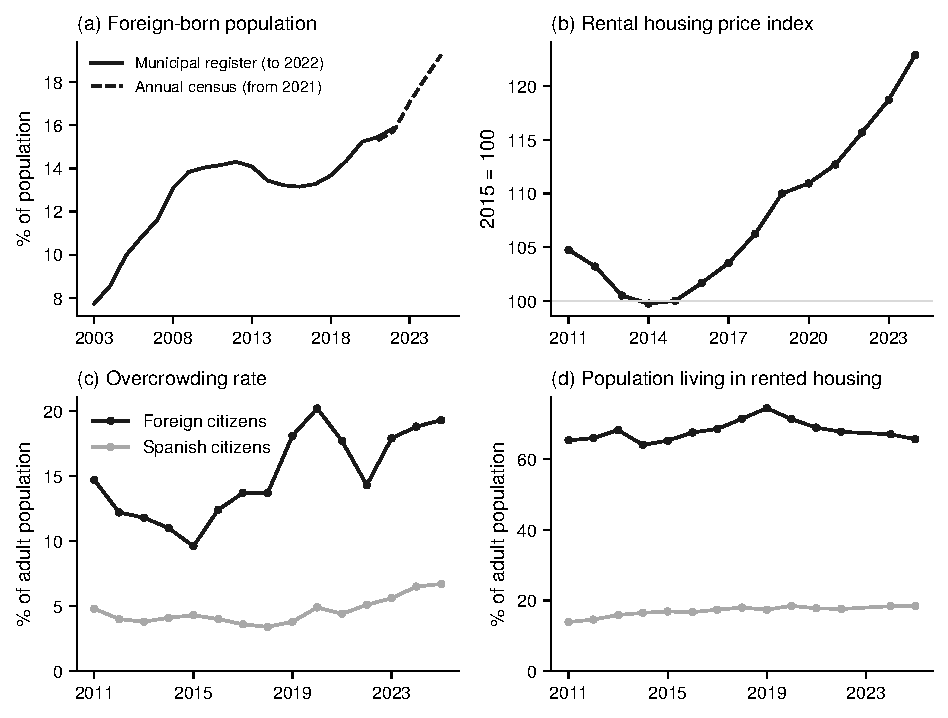
\includegraphics[width=0.94\linewidth]{fig/fig1_contexto.pdf}
\caption{Immigration, rents and housing conditions}\label{fig:context}
\begin{minipage}{0.94\linewidth}\footnotesize\vspace{2pt}
\textit{Notes}: panel (a), foreign-born population on 1 January as a percentage of the population, from the municipal register and the annual population census. Panel (b), national IPVA. Panel (c), percentage of adults living in a dwelling with fewer rooms than required by household size and composition under the Eurostat definition (table ilc\_lvho15). Panel (d), percentage of adults living in rented housing (ilc\_lvps15). Sources: INE and Eurostat (EU-SILC).
\end{minipage}
\end{figure}

\begin{figure}[!htbp]\centering
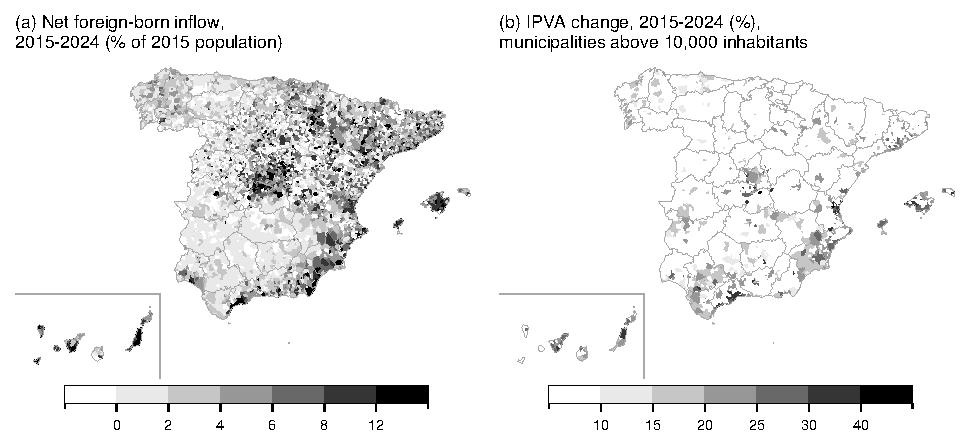
\includegraphics[width=\linewidth]{fig/fig7_mapas.pdf}
\caption{Territorial distribution of immigration and rents}\label{fig:maps}
\begin{minipage}{0.95\linewidth}\footnotesize\vspace{2pt}
\textit{Notes}: panel (a), change in the foreign-born population between 1 January 2015 and 1 January 2024 as a percentage of 2015 population, linked through within-source differences. Panel (b), change in the municipal IPVA between 2015 and 2024; municipalities without an index in white. Sources: INE, IGN.
\end{minipage}
\end{figure}

\subsection{Occupancy is not overcrowding}

Tract-level indicators from the 2011 and 2021 censuses measure, for each municipality, population, foreign-born population, primary and non-primary dwellings, households and tenure; the 2011 census adds population by region of birth, rooms and floor area of primary dwellings. The paper measures \emph{occupancy}, persons per primary dwelling, and, with the annual register and the cadastre, registered population per cadastral dwelling. Neither is a measure of \emph{overcrowding}, which requires rooms relative to household composition; the 2021 census does not report rooms in its tract indicators. The two censuses also define households differently: in 2021 households are built from register entries at each dwelling, and in the tract data the number of households equals the number of primary dwellings in every municipality, so sharing between households cannot be observed in 2021. These differences are a reason to prefer the annual register-cadastre series where possible and to test whether the census measures diverge from it with immigrant exposure.

\subsection{Other data and sample}

Predetermined municipal characteristics come from the 2011 census (population, renting share, non-primary dwellings, share of adults with tertiary education, share aged 65 or more, rooms per dwelling) and from the 2012 INE firm directory (shares of construction, industry and trade-transport-hospitality firms and firms per inhabitant). Eurostat's correspondence of local administrative units provides the coastal indicator and the functional urban area (FUA) and core city of each municipality. Income per person comes from the INE household income atlas, which starts in 2015. The Generalitat de Catalunya publishes the municipalities in tensioned residential market zones and in areas of strong demand; the latter, restricted to municipalities above 20,000 inhabitants, reproduces the 61 municipalities covered by the 2020--2022 rent containment regime. Municipal intermunicipal migration of the Spain-born for 2021--2024 comes from the INE statistics on migrations and changes of residence. Eurostat provides immigration by country of birth into other European countries (appendix A lists all sources, including those that could not be used).

The main sample is a panel of 699 municipalities with an IPVA in 42 provinces with at least two sample municipalities, 9,060 municipality-years between 2012 and 2024 (appendix table~\ref{tab:flow}). Table~\ref{tab:desc} summarises the variables.

\begin{table}[!htbp]\centering\small
\caption{Descriptive statistics of the municipal sample, 2012--2024}\label{tab:desc}
\begin{adjustbox}{max width=\linewidth}\begin{tabular}{lrrrrr}\toprule
 & Mean & Std. dev. & Weighted mean & P10 & P90 \\ \midrule
Annual rent growth (\%) & 1.05 & 2.32 & 1.14 & $-$2.24 & 3.47\\
Foreign-born inflow / population (\%) & 0.34 & 1.01 & 0.46 & $-$0.43 & 1.42\\
Predicted inflow (\%) & 0.39 & 0.98 & 0.48 & $-$0.35 & 1.47\\
Foreign-born share, 2003 (\%) & 8.62 & 8.46 & 8.81 & 1.84 & 18.07\\
Renting households, 2011 (\%) & 13.12 & 6.88 & 15.81 & 5.63 & 22.29\\
Non-primary dwellings, 2011 (\%) & 27.64 & 13.72 & 21.93 & 12.43 & 47.12\\
Tertiary education, 2011 (\%) & 16.46 & 7.17 & 21.19 & 9.73 & 25.96\\
Population aged 65+, 2011 (\%) & 14.80 & 4.24 & 16.16 & 9.36 & 20.01\\
Construction firms, 2012 (\%) & 15.22 & 3.84 & 13.49 & 10.63 & 20.28\\
Trade, transport and hospitality firms, 2012 (\%) & 43.33 & 6.20 & 39.56 & 35.60 & 50.77\\
Coastal municipality (\%) & 41.90 & 49.34 & 44.64 & 0.00 & 100.00\\
FUA core city (\%) & 24.22 & 42.84 & 69.35 & 0.00 & 100.00\\
Persons per room, 2011 & 0.55 & 0.05 & 0.55 & 0.49 & 0.60\\
Population, 2011 & 49,192 & 150,691 & 542,310 & 11,250 & 86,200\\
\bottomrule\end{tabular}\end{adjustbox}
\begin{minipage}{0.95\linewidth}\footnotesize\vspace{4pt}\textit{Notes}: 9,060 municipality-year observations for 699 municipalities in 42 provinces. Flows between consecutive mid-years over population on 1 January of the previous year. The weighted mean uses 2003 population. Sources: INE (IPVA, Padrón, annual population census, 2011 census, firm directory), Eurostat (LAU 2021).\end{minipage}\end{table}

\section{Empirical design}\label{sec:empirics}

\subsection{Specification}

The estimating equation is
\begin{equation}\label{eq:main}
\Delta\ln R_{it}=\beta\, m_{it}+\lambda_{p(i)t}+\sum_{\tau}\mathbf{1}[t=\tau]\big(\phi_\tau S_i+\mathbf{x}_i'\boldsymbol\gamma_\tau\big)+u_{it},
\end{equation}
where $\Delta\ln R_{it}$ is the growth of municipality $i$'s IPVA in year $t$, $m_{it}$ the change in the foreign-born population between mid-year $t-1$ and mid-year $t$ divided by population in January of $t-1$, and $\lambda_{p(i)t}$ province-by-year fixed effects, so that $\beta$ compares municipalities in the same province and year. $S_i$ is the 2003 foreign-born share and $\mathbf{x}_i$ a vector of predetermined characteristics; both are interacted with every year of the sample.\footnote{An earlier version of this paper omitted the interaction for the first year of each estimation sample. This restriction is innocuous in the full sample but not in subsamples: for 2020--2024 it produced an estimate of \wTwoZeroTwoFourold{} instead of \wTwoZeroTwoFour{} (table~\ref{tab:falsification}).}

Four sets of controls are reported. The \emph{minimal} specification includes only $S_i\times$ year. The \emph{original} specification adds log income per person in 2015, log population in 2011 and the 2011 shares of renting households and non-primary dwellings. The \emph{central} specification, defined before estimation in the revision plan, replaces 2015 income, which is measured inside the sample period, by predetermined variables chosen for their link with local housing-demand trends: log population, renting share, non-primary share, tertiary-education share and share aged 65+ in 2011; the 2012 shares of construction, industry and trade-transport-hospitality firms and firms per inhabitant; and coastal and FUA-core indicators, all interacted with year. The fourth adds province $\times$ size class $\times$ year fixed effects, which remove comparisons between the main city of a province and smaller municipalities. Contemporaneous variables such as employment, construction or tourist dwellings are not controlled for because they respond to immigration.

Weights change the estimand. Weighting by 2003 population gives the effect for the typical resident; weighting by rented main dwellings in 2011 gives the effect for the typical renter, the natural estimand for a rent index; unweighted estimates give the effect in the typical municipality. All three are reported, and differences between them are read as heterogeneity rather than resolved by choosing one \citep{solon2015}. Standard errors are clustered by province.

\subsection{Instrument and identifying assumptions}\label{sec:instrument}

The instrument is the inflow predicted by origin networks:
\begin{equation}\label{eq:z}
z_{it}=\sum_{o=1}^{33}s_{io}\,g^{(-p)}_{ot},\qquad s_{io}=\frac{F_{io,2003}}{P_{i,2003}},\qquad g^{(-p)}_{ot}=\frac{\Delta F^{(-p)}_{ot}}{F_{o,2003}},
\end{equation}
where $F_{io,2003}$ is the population born in origin $o$ living in $i$ in 2003 and $\Delta F^{(-p)}_{ot}$ the national change for that origin excluding $i$'s province, with the same timing as the treatment. Its validity can rest on the exogeneity of the shares \citep{goldsmith2020} or on that of the shocks \citep{borusyak2022}. The 2003 shares are correlated with municipal characteristics, which rules out the first reading without further conditioning. The second requires that origin growth be as good as randomly assigned with respect to the exposure-weighted unobserved determinants of rents, $\bar u_{ot}=\sum_i\omega_is_{io}u_{it}/\sum_i\omega_is_{io}$, and that there be many shocks with small weights. Leaving out the own province removes mechanical endogeneity but not pull factors common to many provinces, such as service-sector demand in large cities or the construction cycle. Recentring the instrument by its expectation under permutations of the growth paths across origins \citep{borusyak2023} delivers exact inference if the permutation strata reflect the true assignment process; exchangeability is more plausible within continents and within origins of similar size than across all origins.

\subsection{Inference}

Inference has four layers, each addressing a different threat. Anderson-Rubin (AR) sets with province clusters, analytical and with 4,999 restricted wild-bootstrap draws with Webb weights \citep{davidson2010,roodman2019,webb2023}, are robust to weak instruments and to few clusters of unequal size \citep{mackinnon2023}; with a first-stage $F$ around 30, the conventional $t$-test is not exactly sized \citep{lee2022}, so AR sets are the main inferential object. These sets assume independence across provinces, which shift-share designs violate when municipalities in different provinces share origin compositions. Randomisation inference permutes the growth paths of origins 2,000 times within strata (all origins, terciles of origin size, continents), recentres the instrument and inverts the studentised reduced-form test; it is exact under exchangeability within the strata. Finally, the null-imposed exposure-robust test of \citet{adao2019}, AKM0, treats origin-year shocks as the source of randomness and clusters them by origin, allowing for the serial correlation of each origin's growth; it is computed for the instrument with national shocks, whose 2SLS coefficient equals exactly the shock-level estimate of \citet{borusyak2022}.\footnote{With national shocks the 2SLS coefficient is \natIV{} in the original specification and the exact shock-level equivalent \bhjEq. The shock-level regression reported in the earlier version of the paper (0.23) added year fixed effects at the shock level (\bhjYfe) and used national rather than leave-out shocks, which explains its difference from the leave-out estimate of 0.30.} Multiple endogenous variables are evaluated with \citet{sanderson2016} $F$ statistics.

\subsection{Design diagnostics}

Table~\ref{tab:design} and figure~\ref{fig:shocks} describe the identifying variation. The effective number of origins is \effN, the mean first-order autocorrelation of each origin's annual growth is \autoc{} and the mean pairwise correlation of growth paths is \corrAll{} across all origins (\corrAme{} among American origins, \corrEur{} among European ones): the shocks do not behave as many independent experiments. The Rotemberg decomposition of \citet{goldsmith2020} assigns weights of \rotRom{} to Romania and \rotCol{} to Colombia. Romania's national stock fell by \gRom{} times its 2003 level between 2012 and 2024, so a large part of the identifying variation comes from the departure of Romanians from the municipalities where they had settled during the construction boom; the sum of negative weights is \rotNeg. Using the 33 origin components as separate instruments, the overidentification test rejects ($J$ of \Jstat) and LIML gives \limlB{} (\limlSe), signalling heterogeneous origin-specific effects or invalid components. At the shock level, origins that grew more in 2015--2024 were those whose exposed municipalities had higher renting and tertiary-education shares and, most clearly, a lower share of construction firms (standardised coefficient \balConstr, $p$ = \balConstrP; within continents \balConstrW, $p$ = \balConstrWP). The national shocks are thus related to the economic structure of the municipalities exposed to them, which motivates the central controls.

\begin{table}[!htbp]\centering\small
\caption{Design diagnostics: shocks, Rotemberg weights and shock-level balance}\label{tab:design}
\begin{adjustbox}{max width=\linewidth}\begin{tabular}{lrrrrrr}\toprule
\multicolumn{7}{l}{\textit{A. Origin shocks, 2012--2024 (national growth over the 2003 stock)}}\\
Effective number of origins (inverse HHI of exposure) & 15.8 & \multicolumn{5}{l}{Largest exposure weight: 0.13 (Morocco)}\\
Mean first-order autocorrelation of shocks & 0.64 & \multicolumn{5}{l}{Mean pairwise correlation, all origins: 0.71}\\
Mean correlation within continent & \multicolumn{6}{l}{Europe 0.68, Africa 0.89, Americas 0.85, Asia 0.67}\\
Overidentification with 33 instruments: Hansen $J$ (df) & 137.4 (32) & \multicolumn{5}{l}{$p$-value 0.000; LIML 0.17 (0.09)}\\
\midrule\multicolumn{7}{l}{\textit{B. Largest Rotemberg weights (original specification, population weights)}}\\
Origin & $\hat\alpha_o$ & $\hat\beta_o$ & $F_o$ & Share 2003 & $g_{2012-14}$ & $g_{2015-24}$\\
Romania & 0.314 & 0.39 & 27.0 & 0.042 & $-$1.12 & $-$1.20\\
Colombia & 0.210 & 0.68 & 14.9 & 0.079 & $-$0.07 & 2.41\\
United Kingdom & 0.140 & $-$0.52 & 6.1 & 0.053 & $-$0.64 & $-$0.02\\
Peru & 0.103 & $-$0.05 & 60.1 & 0.022 & $-$0.14 & 3.34\\
Germany & 0.100 & $-$0.54 & 12.1 & 0.057 & $-$0.34 & $-$0.04\\
Ukraine & 0.051 & $-$0.24 & 0.8 & 0.013 & 0.06 & 2.92\\
Venezuela & 0.047 & 1.55 & 2.1 & 0.025 & 0.05 & 6.30\\
Russia & 0.044 & $-$0.02 & 5.6 & 0.009 & 0.44 & 2.06\\
Sum of negative weights & $-$0.166 & \multicolumn{5}{l}{Contribution of the eight largest weights: 0.196 of 0.303}\\
\midrule\multicolumn{7}{l}{\textit{C. Shock-level balance: 2015--2024 origin growth on exposure-weighted characteristics (standardised)}}\\
Characteristic & \multicolumn{2}{c}{Coefficient (s.e.)} & $p$ & \multicolumn{2}{c}{Within continent (s.e.)} & $p$\\
Log population, 2011 & \multicolumn{2}{c}{0.31 (0.26)} & 0.236 & \multicolumn{2}{c}{$-$0.50 (0.50)} & 0.328\\
Renting share, 2011 & \multicolumn{2}{c}{0.59 (0.23)} & 0.018 & \multicolumn{2}{c}{0.06 (0.46)} & 0.896\\
Non-primary share, 2011 & \multicolumn{2}{c}{$-$0.34 (0.17)} & 0.052 & \multicolumn{2}{c}{0.20 (0.22)} & 0.376\\
Tertiary education, 2011 & \multicolumn{2}{c}{0.51 (0.25)} & 0.049 & \multicolumn{2}{c}{0.04 (0.50)} & 0.941\\
Share aged 65+, 2011 & \multicolumn{2}{c}{0.22 (0.25)} & 0.388 & \multicolumn{2}{c}{0.09 (0.33)} & 0.784\\
Coastal & \multicolumn{2}{c}{0.01 (0.29)} & 0.966 & \multicolumn{2}{c}{0.40 (0.31)} & 0.206\\
Construction firms share, 2012 & \multicolumn{2}{c}{$-$0.87 (0.23)} & 0.001 & \multicolumn{2}{c}{$-$1.21 (0.43)} & 0.008\\
Trade-transport-hospitality share, 2012 & \multicolumn{2}{c}{$-$0.34 (0.28)} & 0.221 & \multicolumn{2}{c}{0.42 (0.54)} & 0.446\\
Rent growth 2012--2014 & \multicolumn{2}{c}{0.11 (0.28)} & 0.703 & \multicolumn{2}{c}{0.38 (0.23)} & 0.106\\
\bottomrule\end{tabular}\end{adjustbox}
\begin{minipage}{0.97\linewidth}\footnotesize\vspace{4pt}
\textit{Notes}: panel A uses calendar-year national growth rates $g_{ot}=\Delta F_{ot}/F_{o,2003}$ for 2012--2024 and exposure weights $\sum_i\omega_i s_{io}$; the overidentification test uses the 33 origin components of the instrument as separate instruments (two-step GMM, province clusters). Panel B: decomposition $\hat\beta=\sum_o\hat\alpha_o\hat\beta_o$ of \citet{goldsmith2020} for the leave-out instrument with the original covariates; $F_o$ is the first-stage $F$ of each origin component; $g$ are cumulative growth rates over the 2003 stock. Panel C: 33 origins, weights equal to exposure; heteroskedasticity-robust standard errors; ``within continent adds continent fixed effects.
\end{minipage}\end{table}

\begin{figure}[!htbp]\centering
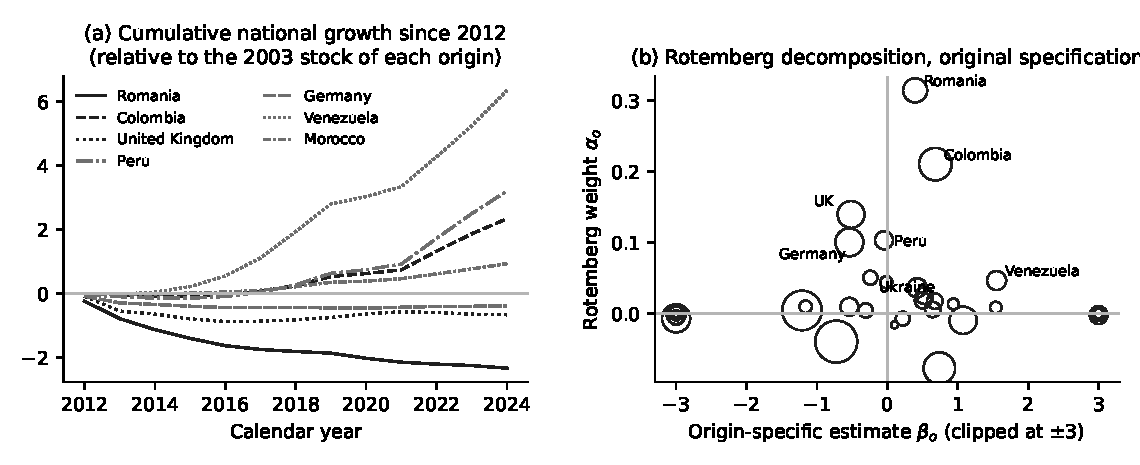
\includegraphics[width=\linewidth]{fig/fig3_shocks.pdf}
\caption{Origin shocks and the Rotemberg decomposition}\label{fig:shocks}
\begin{minipage}{0.95\linewidth}\footnotesize\vspace{2pt}
\textit{Notes}: panel (a), cumulative national growth since 2012 of the largest origins, relative to each origin's 2003 stock. Panel (b), Rotemberg weights $\hat\alpha_o$ and origin-specific estimates $\hat\beta_o$ (clipped at $\pm3$) for the original specification, population weights; circle size proportional to the origin's 2003 share of the foreign-born population.
\end{minipage}
\end{figure}

\section{Effects on rents}\label{sec:rents}

Table~\ref{tab:main} reports the estimates with population weights for the full period and for the arrival period 2015--2024; appendix tables~\ref{tab:main_rent} and \ref{tab:main_unw} report renter-weighted and unweighted estimates, and figure~\ref{fig:forest} summarises them. With minimal controls, an inflow equal to 1\,\% of the population is associated with \minFullB\,\% higher rent growth relative to the province over 2012--2024 (AR set \minFullAR). The original covariates halve the estimate to \origFullB{} (\origFullAR), and the central predetermined controls reduce it further to \cenFullB{} (\cenFullAR). Adding the 2011 tertiary-education and elderly shares to the original covariates is enough to reach a similar value: the original estimate partly reflected trends that differ across municipalities with different education and age structure. Within province $\times$ size cells the estimate is \sizeFullB{} (\sizeFullAR).

\begin{table}[!htbp]\centering\small
\caption{Effect of immigrant inflows on rent growth: estimates and inference (population weights)}\label{tab:main}
\begin{adjustbox}{max width=\linewidth}\begin{tabular}{lcccc}\toprule
 & (1) Minimal & (2) Original & (3) Central & (4) Central + size FE \\ \midrule
\multicolumn{5}{l}{\textit{A. Full period, 2012--2024}}\\
OLS & 0.16 & 0.07 & 0.07 & 0.06 \\
Reduced form & 0.30 & 0.11 & 0.05 & 0.01 \\
First-stage $F$ & 34.5 & 32.2 & 29.0 & 30.0 \\
2SLS & 0.55 & 0.30 & 0.13 & 0.01 \\
 & (0.13) & (0.12) & (0.10) & (0.13) \\
AR 95\% set, province clusters & [0.33, 0.87] & [0.09, 0.58] & [$-$0.08, 0.35] & [$-$0.23, 0.30] \\
AR 95\% set, wild bootstrap & [0.31, 0.90] & [0.03, 0.59] & [$-$0.15, 0.36] & [$-$0.31, 0.32] \\
Randomisation, all origins & [0.37, 0.76] & [0.15, 0.44] & [0.02, 0.26] & [$-$0.10, 0.24] \\
Randomisation, size terciles & [0.24, 0.82] & [0.07, 0.48] & [$-$0.05, 0.36] & [$-$0.18, 0.39] \\
Randomisation, within continents & $(-\infty,\infty)$ & $(-\infty,\infty)$ & $(-\infty,\infty)$ & $(-\infty,\infty)$ \\
2SLS with national shocks & 0.49 & 0.22 & 0.10 & 0.00 \\
AKM0 95\% set, shocks clustered by origin & [0.31, 1.04] & [$-$0.08, 0.90] & [$-$0.65, 0.44] & [$-$0.78, 0.54] \\
Observations & 9,060 & 9,060 & 9,060 & 8,449 \\
\midrule
\multicolumn{5}{l}{\textit{B. Arrival period, 2015--2024}}\\
OLS & 0.23 & 0.12 & 0.12 & 0.12 \\
Reduced form & 0.31 & 0.14 & 0.09 & 0.05 \\
First-stage $F$ & 22.8 & 14.6 & 14.4 & 16.4 \\
2SLS & 0.62 & 0.45 & 0.24 & 0.13 \\
 & (0.15) & (0.16) & (0.11) & (0.12) \\
AR 95\% set, province clusters & [0.38, 1.05] & [0.21, 0.99] & [0.07, 0.59] & [$-$0.06, 0.52] \\
AR 95\% set, wild bootstrap & [0.40, 1.50] & [0.19, 0.96] & [0.06, 0.59] & [$-$0.07, 0.51] \\
Randomisation, all origins & [0.46, 0.84] & [0.28, 0.62] & [0.15, 0.34] & [0.06, 0.28] \\
Randomisation, size terciles & [0.39, 0.88] & [0.26, 0.64] & [0.13, 0.43] & [0.03, 0.35] \\
Randomisation, within continents & $(-\infty,\infty)$ & [$-\infty$, 1.16] & [$-\infty$, 1.00] & $(-\infty,\infty)$ \\
2SLS with national shocks & 0.57 & 0.36 & 0.20 & 0.13 \\
AKM0 95\% set, shocks clustered by origin & [0.41, 3.21] & [0.13, $\infty$] & [$-$0.56, 0.82] & [$-$0.68, 0.52] \\
Observations & 6,972 & 6,972 & 6,972 & 6,502 \\
\bottomrule
\end{tabular}\end{adjustbox}
\begin{minipage}{0.97\linewidth}\footnotesize\vspace{4pt}
\textit{Notes}: dependent variable $\Delta\ln R_{it}$, annual growth of the municipal IPVA; treatment $m_{it}$, foreign-born inflow over population (centred timing); instrument $z_{it}$, 2003 shares of 33 origins times national growth excluding the own province. All columns include province $\times$ year fixed effects and the 2003 foreign-born share interacted with every year. Column 2 adds the original covariates (log income per person 2015, log population 2011, 2011 shares of renting households and non-primary dwellings) $\times$ year; column 3 replaces them with the central set of predetermined covariates (2011 census: log population, renting share, non-primary share, tertiary-education share, share aged 65+; 2012 firm directory: shares of construction, industry and trade-transport-hospitality firms and firms per capita; coastal and FUA-core indicators) $\times$ year; column 4 adds province $\times$ size class $\times$ year fixed effects. Anderson-Rubin (AR) sets invert the reduced-form test with province-clustered errors (analytical) or with 4,999 restricted wild-bootstrap draws with Webb weights. Randomisation sets permute the growth paths of origins 2,000 times within the indicated strata, recentre the instrument and invert the studentised reduced-form test. The last two rows use national (not leave-out) shocks; AKM0 is the null-imposed exposure-robust test of \citet{adao2019} with origin-year shocks clustered by origin. $\infty$ denotes an unbounded set. Weights: 2003 population.
\end{minipage}\end{table}

The full-period estimate averages two different regimes. In 2012--2014 the foreign-born population fell, and the predicted outflows are not associated with rent changes (table~\ref{tab:falsification}); in the arrival years 2015--2024 the central specification gives \cenArrB{} (standard error \cenArrSe, first-stage $F$ \cenArrF), with an AR set of \cenArrAR{} and a wild-bootstrap AR set of \cenArrWCR. With renter weights the estimate is \cenArrRB{} (\cenArrRAR), and unweighted \cenArrUB{} with an uninformative set (\cenArrUAR). Within province $\times$ size cells it falls to \sizeArrB{} (\sizeArrAR). The arrival-period estimate of the central specification excludes zero under province-clustered AR and wild-bootstrap inference and under randomisation across all origins (\cenArrRI, $p$ = \cenArrRIp{} for $\beta=0$), but not under randomisation within continents (\cenArrRIcont) or under the AKM0 test with shocks clustered by origin (\cenArrAKM). Which of these is appropriate depends on whether the growth paths of Latin American, African and European origins can be treated as exchangeable; the diagnostics in table~\ref{tab:design} make that assumption hard to defend, and within-continent variation alone does not bound the effect.

\begin{figure}[!htbp]\centering
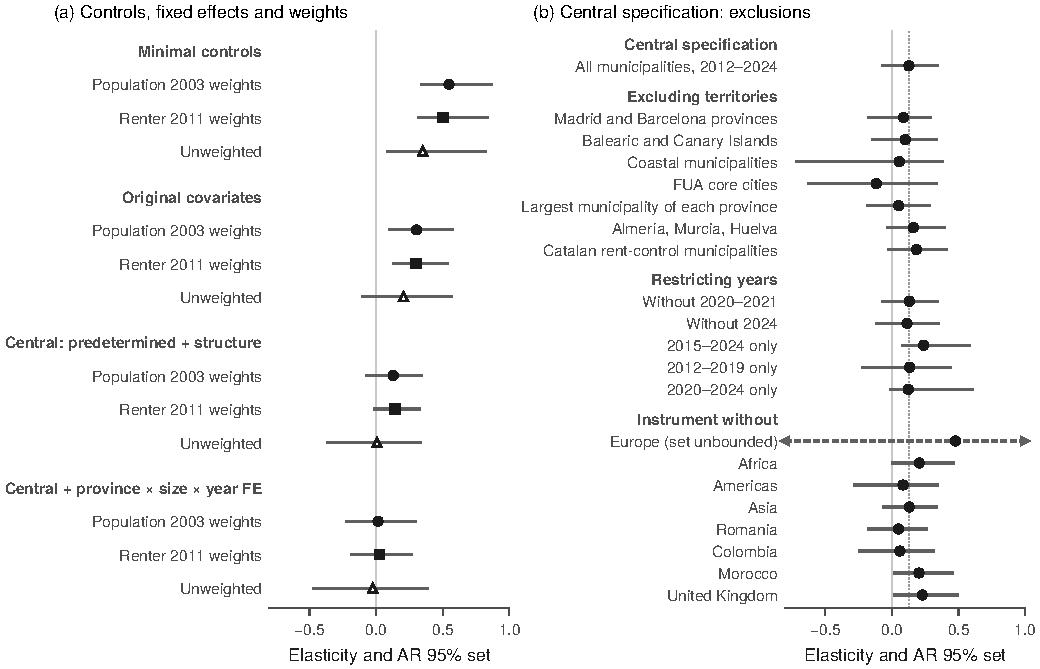
\includegraphics[width=\linewidth]{fig/fig4_forest.pdf}
\caption{Rent elasticity across specifications, weights and exclusions}\label{fig:forest}
\begin{minipage}{0.95\linewidth}\footnotesize\vspace{2pt}
\textit{Notes}: point estimates and analytical Anderson-Rubin 95\,\% sets (province clusters), 2012--2024, truncated to $[-1,1.5]$. Panel (a): specifications of table~\ref{tab:main} with the three weighting schemes. Panel (b): central specification, population weights, excluding territories, periods or origins (the excluded origin is removed from the instrument and from the exposure control); appendix table~\ref{tab:loo} summarises all leave-one-out estimates.
\end{minipage}
\end{figure}

The OLS coefficient is smaller than the 2SLS estimate in most columns. A smaller OLS coefficient is consistent with newcomers choosing municipalities where rents would otherwise grow less, but also with measurement error in registered inflows; it does not by itself validate the instrument.

The exclusions in figure~\ref{fig:forest} show that the central estimate is not driven by a single province, autonomous community or origin (appendix table~\ref{tab:loo}), but that it is smaller, and close to zero, without FUA core cities, without coastal municipalities or without the largest municipality of each province: the comparisons between main cities and their surroundings carry much of the identifying variation. Spatial spillovers to contiguous municipalities or distance rings are small and imprecise (appendix table~\ref{tab:altspatial}): for contiguous municipalities, \spContig{} (standard error \spContigSe). The design does not detect spillovers, but their confidence intervals do not exclude effects of the order of the own effect.

\section{Validity}\label{sec:validity}

\subsection{Pre-periods and placebo outcomes}

The IPVA starts in 2011, so there is no rent pre-period before the sample. Table~\ref{tab:falsification} uses three alternatives. First, rent growth in 2011--2014 is regressed on the inflow predicted for 2015--2024, controlling for the inflow predicted for 2011--2014. With the central controls the coefficient is \preW{} (standard error \preWse, $p$ = \preWp): municipalities more exposed to the later shocks had, if anything, slower rent growth before them. The 2015--2024 reduced form with the same controls is \rfLDW{} (\rfLDWse). The pre-period coefficient is not significant at 5\,\%, but its magnitude is comparable to that of the reduced form and of opposite sign, a pattern consistent with a post-crisis recovery in the more exposed municipalities that would bias the arrival-period estimate upwards. This threat cannot be ruled out with the available data. Second, with the original covariates the predicted 2015--2024 inflow also predicts faster growth of the Spain-born population in 2003--2008 (coefficient \natPreOrig, $p$ = \natPreOrigP), a sign of pre-existing differences in demographic dynamics; the central controls remove it (\natPreCen, $p$ = \natPreCenP). Third, reassigning the 2003 share vectors at random across municipalities of the same province and size class produces reduced forms as large as the observed one in a large fraction of draws ($p$ = \permP), and origin shares predicted from observable characteristics reproduce the observed reduced form. Under the central specification, the variation that the instrument adds to municipal characteristics is therefore modest.

\begin{table}[!htbp]\centering\small
\caption{Falsification, dynamics and stability}\label{tab:falsification}
\begin{adjustbox}{max width=\linewidth}\begin{tabular}{lcc}\toprule
 & Population weights & Unweighted \\ \midrule
\multicolumn{3}{l}{\textit{A. Pre-period and placebo outcomes (cross-section of municipalities)}}\\
Rent growth 2011--2014 on predicted 2015--2024 inflow (original controls) & $-$0.124 (0.070) & $-$0.089 (0.052)\\
Rent growth 2011--2014 on predicted 2015--2024 inflow (central controls) & $-$0.085 (0.046) & $-$0.056 (0.046)\\
\quad Reference: rent growth 2015--2024 on the same instrument (central controls) & 0.102 (0.043) & 0.067 (0.050)\\
Spain-born growth 2003--2008 (original controls) & 0.408 (0.135) & 0.754 (0.325)\\
Spain-born growth 2003--2008 (central controls) & $-$0.011 (0.081) & 0.109 (0.192)\\
Spain-born growth 2008--2011 (central controls) & $-$0.006 (0.032) & $-$0.061 (0.081)\\
Reduced form with permuted share vectors (province $\times$ size cells): $p$-value of observed & 0.35 & --\\
Reduced form with pseudo-shares predicted from observables vs observed & 0.050 vs 0.054 & --\\
\midrule\multicolumn{3}{l}{\textit{B. Dynamics and persistence of the instrument (original covariates, population weights)}}\\
Correlation of predicted inflows: 2003--2008 with 2015--2024 & 0.74 & 0.58\\
2SLS adding predicted 2003--08 and 2008--12 inflows $\times$ year & 0.29 (0.14), $F$ 11.9 & --\\
Local projections, balanced 2015--2020: joint test of leads, $p$ (original / minimal) & 0.65 / 0.62 & 0.85 / 0.70\\
\quad First-stage $F$ of the instrument innovation (original / minimal) & 2.8 / 6.8 & 0.5 / 0.8\\
Two-instrument model: current / previous calendar-year inflow & $-$0.00 / 0.09 & --\\
\quad Sanderson-Windmeijer $F$ & 8.7 / 34.1 & --\\
Same sample 2013--2024: centred / calendar-year / calendar with lagged instrument & 0.31 / 0.05 / $-$0.03 & --\\
\quad with municipality fixed effects (centred) & 0.48 ($F$ 4.7) & --\\
\midrule\multicolumn{3}{l}{\textit{C. Stability and symmetry (original covariates, all year interactions, population weights)}}\\
Window 2012--2014 (net outflows) & $-$0.01 (0.26), AR [$-$0.49, 0.57] & --\\
Window 2015--2024 (arrivals) & 0.45 (0.16), AR [0.21, 0.99] & --\\
Window 2012--2019 & 0.30 (0.15), AR [$-$0.02, 0.59] & --\\
Window 2020--2024 & 0.31 (0.19), AR [0.05, 2.28] & --\\
2020--2024 omitting the first-year interaction (as in the original manuscript) & $-$0.46 (0.29) & --\\
Observations with positive / non-positive predicted inflow & 0.53 (0.23) / 0.04 (0.20) & --\\
Controlling for Catalan rent-control and tensioned-zone municipalities $\times$ year & 0.30 (0.13) & --\\
\bottomrule\end{tabular}\end{adjustbox}
\begin{minipage}{0.97\linewidth}\footnotesize\vspace{4pt}
\textit{Notes}: panel A regresses the indicated outcome on the predicted 2015--2024 inflow (2003 shares, leave-province-out national growth), with province fixed effects, the 2003 foreign-born share and the indicated controls; the 2011--2014 regressions also control for the predicted 2011--2014 inflow. Permuted shares: 300 reassignments of the 2003 share vectors across municipalities within province $\times$ size cells (central specification). Pseudo-shares: origin shares predicted from the central covariates with province fixed effects. Panel B: local projections of $\ln R_{t+h}-\ln R_{t-1}$ on the calendar-year inflow instrumented with its prediction, controlling for three lags of the prediction, balanced sample $t\in[2015,2020]$, $h\in\{-4,\dots,4\}$; the joint test covers $h\in\{-4,-3,-2\}$. Panel C: subsample estimates with every year interaction of the controls. Standard errors clustered by province.
\end{minipage}\end{table}

\subsection{Dynamics and the persistence of migration flows}

The 2003 shares predict both the boom-era inflows and the post-2015 inflows: the correlation of the predicted inflows of 2003--2008 and 2015--2024 across sample municipalities is \boomCorr. Controlling for the boom and bust predictions interacted with year leaves the original estimate little changed but weakens the first stage. Separating short- and long-run responses as proposed by \citet{jaeger2018} requires variation in the instrument's innovations, and there is little: in a balanced sample of 2015--2020, controlling for three lags of the prediction, the first-stage $F$ of the innovation is \lpFcov{} with the original covariates and \lpFmin{} with minimal controls (appendix figure~\ref{fig:lp}). Joint tests of the leads do not reject, but with such weak first stages they have little power and do not validate the design. The two-instrument model gives a Sanderson-Windmeijer $F$ of \swFOne{} for the current inflow and does not separate the current and lagged responses. The timing of the treatment also matters: in the same sample, the centred inflow, which averages arrivals registered by January of $t$ and during $t$, gives \cenB, while the inflow registered during calendar year $t$ gives \calB. Declared rents in year $t$ are associated with arrivals registered by the beginning of the year, not with those of the same calendar year. The paper therefore makes no claim on whether the relative effect persists or dissipates.

\subsection{Stability, symmetry and policy}

The response differs between periods of outflows and of arrivals (panel C of table~\ref{tab:falsification}). With the original covariates and every year interaction, the estimate is \wOut{} (\wOutSe) in 2012--2014, when the predicted inflow was mostly negative, and \wIn{} (\wInAR) in 2015--2024; observations with positive predicted inflows drive the estimate. An index of contracts in force with nominal rigidity can plausibly respond more to arrivals than to departures, and pooling both regimes understates the response to arrivals. The estimate for 2020--2024 is positive (\wTwoZeroTwoFour, AR set \wTwoZeroTwoFourAR) once every year interaction is included; the negative estimate reported in an earlier version of this paper reflected the omission of the 2020 interactions. Controlling for the Catalan municipalities under rent containment in 2020--2022 and in tensioned zones from 2024, or excluding them, does not reduce the estimates.

\subsection{A sharper episode: the 2016 visa waivers for Colombia and Peru}

The Schengen visa requirement for Colombian citizens was lifted in December 2015 and that for Peruvian citizens in March 2016, after which arrivals from both countries accelerated. The episode offers variation with a known date that is driven by policy in the origin countries rather than by Spanish demand, and it can be exploited within a continent: the regressions compare municipalities with the same 2003 exposure to other American origins, removing the contrast between Latin American, African and European settlement that drives the full instrument. Table~\ref{tab:episode} and figure~\ref{fig:episode} show the results. The foreign-born stock rises from 2017 in municipalities more exposed to Colombian and Peruvian settlement, with no pre-trend, and rents follow with no pre-trend. With population weights the implied elasticity is \epBW{} (standard error \epSeW, first-stage $F$ \epFW), with an AR set of \epARW{} and a wild-bootstrap set of \epWCRW; with renter weights it is \epBR{} (\epWCRR). Without weights the first stage is weak ($F$ \epFU) and the estimate, \epBU, is uninformative. The episode supports a positive relative effect of arrivals on rents in the large municipalities where Colombian and Peruvian immigrants settled, of a size comparable to or larger than the shift-share estimates, but it rests on a moderately weak first stage and on a single pair of origins. Episodes for Venezuela and Ukraine do not provide a usable design: the Venezuelan first stage is weak and Ukrainian exposure shows strong pre-trends.

\begin{table}[!htbp]\centering\small
\caption{A sharper episode: the 2016 Schengen visa waivers for Colombia and Peru}\label{tab:episode}
\begin{adjustbox}{max width=\linewidth}\begin{tabular}{lccc}\toprule
 & Population weights & Renter weights & Unweighted\\\midrule
\multicolumn{4}{l}{\textit{A. Difference-in-differences IV, 2011--2024 (exposure: 2003 Colombian and Peruvian share, pp)}}\\
First stage: foreign-born stock (pp) on exposure $\times$ post & 0.90 (0.29) & 1.05 (0.34) & 0.90 (0.43)\\
First-stage $F$ & 9.4 & 9.4 & 4.3\\
Rent (\%) per pp of inflow & 0.64 (0.20) & 0.68 (0.18) & 0.27 (0.24)\\
AR 95\% set, province clusters & [0.22, 1.27] & [0.31, 1.25] & [$-$1.68, 1.27]\\
AR 95\% set, wild bootstrap & [0.04, 1.80] & [0.10, 1.92] & $(-\infty,\infty)$\\
\midrule\multicolumn{4}{l}{\textit{B. Event-study averages (coefficients per pp of exposure; pre: $k\le-2$, post: $k\ge0$)}}\\
Colombia and Peru, 2016: inflow pre / post & $-$0.26 / 0.90 & -- & $-$0.06 / 0.90\\
\quad rent (log points) pre / post & 0.0007 / 0.0058 & -- & $-$0.0007 / 0.0025\\
Venezuela, 2017: inflow pre / post & $-$0.07 / 0.19 & -- & $-$0.12 / 0.14\\
\quad rent (log points) pre / post & 0.0035 / 0.0032 & -- & 0.0054 / 0.0049\\
Ukraine, 2022: inflow pre / post & 1.45 / 0.33 & -- & 0.57 / 0.36\\
\quad rent (log points) pre / post & 0.0050 / 0.0005 & -- & 0.0059 / $-$0.0018\\
\bottomrule\end{tabular}\end{adjustbox}
\begin{minipage}{0.97\linewidth}\footnotesize\vspace{4pt}
\textit{Notes}: the exposure is the 2003 share of the population born in the episode countries (pp); all regressions control for the 2003 share born in other countries of the same continent interacted with every event year, so that identification compares municipalities with similar continental exposure. All include province $\times$ year fixed effects and the central covariates $\times$ year. Panel A: outcome $100(\ln R_{it}-\ln R_{i,2015})$, endogenous variable the change in the foreign-born stock since 2015 in pp of 2003 population, instrument exposure $\times$ 1[$t\ge2016$]; exposure is interacted with pre-2016 years so that pre-trends are absorbed. Panel B: averages of event-time coefficients (base year $t_X-1$). Standard errors clustered by province.
\end{minipage}\end{table}

\begin{figure}[!htbp]\centering
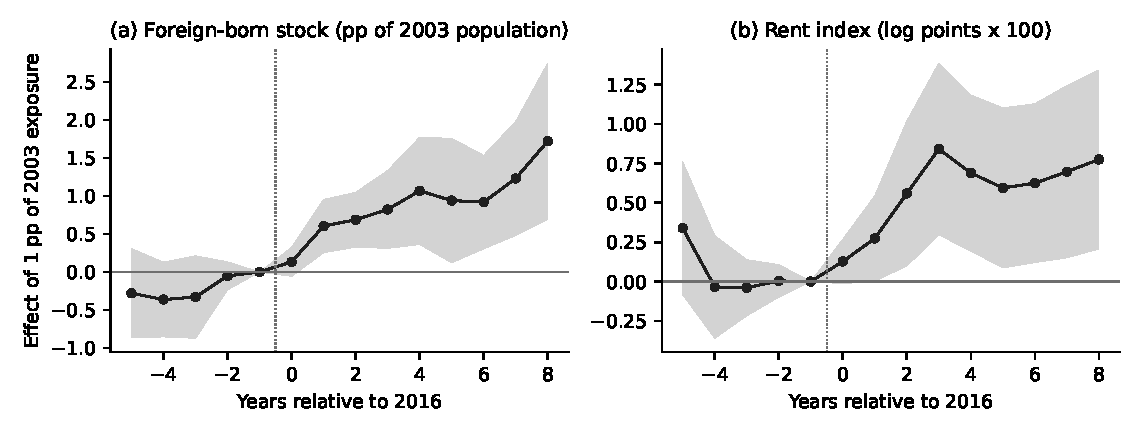
\includegraphics[width=\linewidth]{fig/fig5_event_colper.pdf}
\caption{The 2016 visa waivers for Colombia and Peru: event study}\label{fig:episode}
\begin{minipage}{0.95\linewidth}\footnotesize\vspace{2pt}
\textit{Notes}: coefficients on the 2003 share of the population born in Colombia or Peru (pp) interacted with event years, relative to 2015, controlling for the 2003 share born in other American countries interacted with event years, province $\times$ year fixed effects and the central covariates $\times$ year; population weights; 95\,\% intervals with province clusters.
\end{minipage}
\end{figure}

\subsection{Alternative push shocks}

Replacing the Spanish national growth of each origin by its inflows into twelve other European countries, which reflect push factors common to destinations, would remove Spanish pull factors from the shocks. The resulting instrument has no predictive power for municipal inflows in Spain once exposure and covariates are controlled for (first-stage $F$ of \altF; appendix table~\ref{tab:altspatial}), so this design cannot be used.

\section{Where newcomers are housed}\label{sec:margins}

\subsection{Census decomposition}

Table~\ref{tab:margins} and figure~\ref{fig:margins} estimate identity \eqref{eq:identity} between the 2011 and 2021 censuses, with all components estimated jointly. In the central specification each additional immigrant is associated with \popC{} additional net residents (standard error \popCse) and with \crowdC{} persons housed through higher occupancy of primary dwellings (\crowdCse); the log of persons per primary dwelling rises by \dlnsC{} per unit of inflow. Non-primary dwellings brought into use contribute \vacC{} (\vacCse) and new dwellings \newC{} (\newCse): both supply components are imprecise because the 2011 and 2021 censuses count dwellings differently. The occupancy coefficient is stable across specifications and weights, but the share of net population growth that it represents is not: \shareC{} in the central weighted specification, with a Fieller interval \citep{fieller1954} of \shareCfi{} and a province-bootstrap interval of \shareCbo; \shareA{} with the original covariates (\shareAfi); \shareAU{} and \shareCU{} without weights; and above one with minimal controls, because net residents then barely respond. The data support a substantial role for higher occupancy, not a precise share.

\begin{table}[!htbp]\centering\small
\caption{Where newcomers are housed: margins of adjustment}\label{tab:margins}
\begin{adjustbox}{max width=\linewidth}\begin{tabular}{lcccc}\toprule
 & \multicolumn{2}{c}{Original covariates} & \multicolumn{2}{c}{Central covariates}\\\cmidrule(lr){2-3}\cmidrule(lr){4-5}
 & Weighted & Unweighted & Weighted & Unweighted\\\midrule
\multicolumn{5}{l}{\textit{A. Census long differences 2011--2021 (municipalities above 5,000 inhabitants; persons per immigrant)}}\\
Net residents & 0.80 (0.21) & 1.21 (0.28) & 0.70 (0.24) & 0.61 (0.30)\\
Born in Spain & $-$0.20 (0.21) & 0.21 (0.28) & $-$0.30 (0.24) & $-$0.39 (0.30)\\
New dwellings & $-$0.47 (0.50) & $-$0.80 (0.94) & $-$0.74 (0.55) & $-$1.13 (1.12)\\
Non-primary dwellings brought into use & 0.82 (0.54) & 1.56 (0.90) & 1.00 (0.50) & 1.38 (1.04)\\
Higher persons per primary dwelling & 0.45 (0.15) & 0.45 (0.16) & 0.45 (0.15) & 0.37 (0.18)\\
Persons in dwellings switched to renting & 0.22 (0.08) & 0.41 (0.08) & 0.19 (0.09) & 0.38 (0.10)\\
$\Delta\ln$ persons per primary dwelling & 0.46 (0.15) & 0.46 (0.16) & 0.46 (0.15) & 0.38 (0.18)\\
First-stage $F$ & 38.0 & 14.6 & 30.4 & 11.3\\
Share of net residents absorbed by occupancy & 0.56 & 0.37 & 0.64 & 0.60\\
\quad Fieller 95\% interval & [0.23, 1.02] & [0.14, 0.65] & [0.34, 1.19] & [0.04, 7.95]\\
\quad Province bootstrap 95\% interval & [0.14, 1.20] & [0.18, 0.79] & [$-$0.53, 1.73] & [$-$1.26, 2.83]\\
$\Delta\ln$ persons per dwelling predicted by continental composition & $-$0.08 (0.01) & $-$0.09 (0.02) & $-$0.08 (0.01) & $-$0.09 (0.03)\\
Within-group change (observed minus composition) & 0.54 (0.16) & 0.55 (0.17) & 0.54 (0.16) & 0.47 (0.19)\\
Census minus register-cadastre occupancy, 2021 & -- & -- & $-$0.20 (0.49) & $-$0.74 (0.76)\\
\midrule\multicolumn{5}{l}{\textit{B. Annual register and cadastre, 2015--2023 (central covariates; per unit of calendar-year inflow)}}\\
 & Population weights & Renter weights & Unweighted & \\
$\Delta\ln$ registered population & 0.72 (0.16) & 0.73 (0.17) & 0.38 (0.55) & \\
$\Delta\ln$ cadastral dwellings & $-$0.24 (0.16) & $-$0.26 (0.18) & $-$0.59 (0.50) & \\
$\Delta\ln$ population per cadastral dwelling & 0.96 (0.12) & 0.99 (0.15) & 0.97 (0.32) & \\
First-stage $F$ & 4.9 & 7.2 & 1.5 & \\
\midrule\multicolumn{5}{l}{\textit{C. Spain-born intermunicipal migration, 2021--2024 (INE EMCR; per unit of calendar-year inflow)}}\\
 & Population weights & Unweighted & & \\
Out-migration rate of the Spain-born & $-$0.05 (0.19) & $-$0.43 (0.35) & & \\
In-migration rate of the Spain-born & $-$0.54 (0.41) & $-$1.30 (0.90) & & \\
Net rate & $-$0.49 (0.29) & $-$0.88 (0.68) & & \\
First-stage $F$ & 3.5 & 1.7 & & \\
\bottomrule\end{tabular}\end{adjustbox}
\begin{minipage}{0.97\linewidth}\footnotesize\vspace{4pt}
\textit{Notes}: panel A: each row is a 2SLS regression, estimated jointly across rows (stacked influence functions, province clusters), of the indicated component of identity \eqref{eq:identity} (persons per 2011 inhabitant) on the change in the foreign-born population 2011--2021 per 2011 inhabitant, instrumented with the predicted 2012--2021 inflow; province fixed effects. Rows 1 and 3--5 add up to row 1 by construction. The share is the ratio of rows 5 and 1 with a Fieller interval and a 999-draw province pairs bootstrap. The composition-predicted change holds group-specific dwellings per person fixed at the 2011 ecological estimates (census tracts with municipality fixed effects, table~\ref{tab:kappa}) for Spain-born, European, African, American, Asian and Oceanian residents and applies the 2011 (register) and 2021 (annual census) population shares. Panel B: annual changes on the January-to-January foreign-born inflow instrumented with its prediction, province $\times$ year fixed effects. Panel C: INE Statistics on Migrations and Changes of Residence, municipal tables 69744 and 69746, rates over the Spain-born population on 1 January.
\end{minipage}\end{table}

\begin{figure}[!htbp]\centering
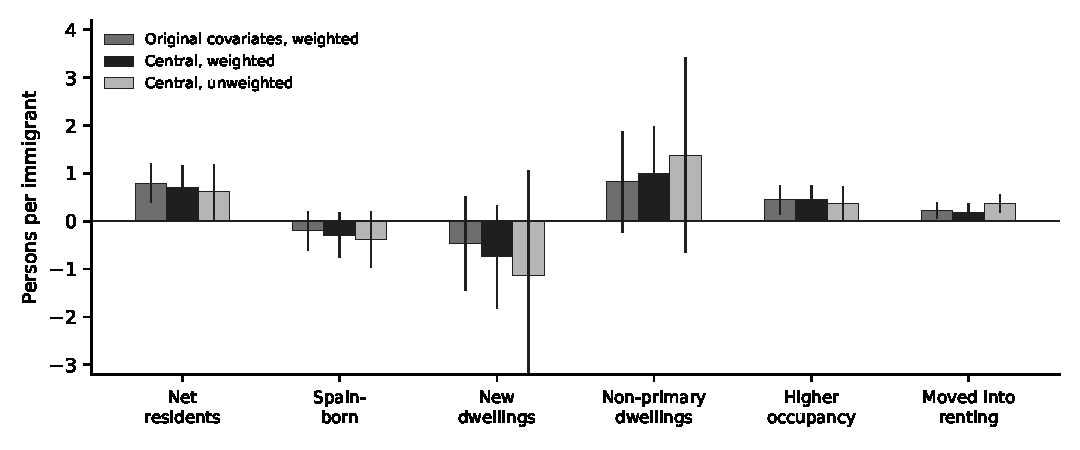
\includegraphics[width=0.9\linewidth]{fig/fig6_margins.pdf}
\caption{Where each immigrant is housed: decomposition 2011--2021}\label{fig:margins}
\begin{minipage}{0.9\linewidth}\footnotesize\vspace{2pt}
\textit{Notes}: 2SLS coefficients of table~\ref{tab:margins}, panel A, with 95\,\% intervals (province clusters). New dwellings, non-primary dwellings and higher occupancy add up to net residents.
\end{minipage}
\end{figure}

\subsection{Composition or more intensive use?}

Higher average occupancy can arise because newcomers live in larger households than the residents they join (composition) or because households of a given group become denser. The 2011 census tracts give dwellings per person by region of birth (appendix table~\ref{tab:kappa}): relative to the average resident, the African-born occupy \kapAfr{} times as many dwellings per person, the Asian-born \kapAsi, the American-born \kapAme{} and the European-born \kapEur. Holding these rates fixed and applying the 2011 and 2021 population shares by region of birth, the change in composition associated with the predicted inflow would \emph{lower} occupancy slightly (\compC), because the identifying variation includes the departure of European-born residents, who occupy more dwellings per person, and the arrival of Latin Americans, whose 2011 rate is close to the average. The observed rise in occupancy is therefore not explained by composition across continental groups. Two caveats apply: the group rates are ecological estimates, and they describe the 2011 stock; recent arrivals of the same continent are likely to live in denser households than settled immigrants \citep{myerslee1996}, a composition effect within groups that these data cannot separate from a denser use of dwellings by all households.

\subsection{Register, cadastre and natives}

With consistent annual sources, registered population per cadastral dwelling rises by \ratioP{} per unit of calendar-year inflow (standard error \ratioPse) and the cadastral stock does not respond (\stockP, \stockPse), in the central specification with population weights (panel B); the first stage of the calendar-year inflow is weak in this specification ($F$ \panelF), so these coefficients are indicative. The ratio of population to the total stock rises when population grows and the stock does not, whether newcomers fill previously vacant dwellings or crowd into occupied ones; it confirms absorption within the registered stock, not higher occupancy as such. The difference between census and register-cadastre occupancy in 2021 is not related to the predicted inflow (panel A, last row), which suggests that the change in census methodology does not drive the occupancy results.

The response of the Spain-born population in the census decomposition is \natC{} per immigrant and not significant. The change in the Spain-born population includes births to immigrant parents and deaths, which the municipal data available for this paper do not separate. Municipal flows of intermunicipal migration for 2021--2024 (panel C) give an out-migration response of the Spain-born of \outES{} (\outESse), with a weak first stage ($F$ \outESF): the data do not identify whether natives relocate.

\subsection{Occupancy and welfare}

Higher occupancy is an adjustment margin that rent indices do not capture. It is not, by itself, evidence of a welfare loss. Occupying previously vacant dwellings uses an idle stock; denser households may reflect preferences, networks, temporary stays or saving, as well as affordability constraints, documentation barriers or discrimination in access to rentals. Distinguishing these requires rooms, household composition, income and, ideally, outcomes such as health or schooling at the local level, which the available data do not provide. National EU-SILC data show that overcrowding among foreign adults rose after 2015 (figure~\ref{fig:context}), but they cannot be linked to local inflows.

\section{Magnitudes: from local to aggregate}\label{sec:magnitude}

The design identifies the effect of an inflow into a municipality relative to its province. Translating it into a national counterfactual requires four assumptions that the design does not test: (A1) that the national elasticity equals the within-province one, which holds in the model of section~\ref{sec:model} only as a lower bound and whose relation to the national effect outside the model is unknown, because province fixed effects remove the common effect of immigration \citep{chodorowreich2020,wolf2023}; (A2) that level effects are permanent, which the dynamics cannot establish; (A3) that the 2015--2024 origin mix has the elasticity implied by the identifying variation, although the overidentification test rejects homogeneity across origins; and (A4) that there are no general-equilibrium effects, for instance through the supply of construction labour or incomes.

Under these assumptions the implied share of national IPVA growth is $\beta\times M/G$, with $M=6.5$\,\% the cumulative net foreign-born inflow relative to population and $G=20.6$ log points the growth of the national IPVA between 2015 and 2024. Table~\ref{tab:magnitude} and figure~\ref{fig:magnitude} report it for several estimates. The central arrival-period estimate implies \shareArr\,\%, with a range of \shareArrLo{} to \shareArrHi\,\% across its AR set; the central full-period estimate implies \shareFull\,\%, with an upper bound of \shareFullHi\,\%; the original specification implied \shareOrig\,\%, and the visa-waiver episode \shareEp\,\%. Across these estimates immigration accounts for a minority of the rise in the rent index, but the figures depend on assumptions that cannot be verified and should not be read as lower bounds. Because the IPVA is a stock index, the corresponding shares for entry rents may differ.

\begin{table}[!htbp]\centering\small
\caption{Implied contribution of immigration to national rent-index growth, 2015--2024, under explicit assumptions}\label{tab:magnitude}
\begin{adjustbox}{max width=\linewidth}\begin{tabular}{lccc}\toprule
Elasticity used & $\beta$ & Robust 95\% set for $\beta$ & Implied share of IPVA growth (\%)\\\midrule
Central specification, 2012--2024 & 0.13 & [$-$0.08, 0.35] & 4.1 \; [0, 11.0]\\
Central specification, arrival period 2015--2024 & 0.24 & [0.07, 0.59] & 7.5 \; [2.2, 18.6]\\
Central, renter weights, 2015--2024 & 0.20 & [0.06, 0.47] & 6.2 \; [1.9, 14.8]\\
Central + province $\times$ size FE, 2015--2024 & 0.13 & [$-$0.06, 0.52] & 4.2 \; [0, 16.4]\\
Original covariates, 2012--2024 & 0.30 & [0.09, 0.58] & 9.6 \; [2.8, 18.3]\\
Colombia--Peru episode (DiD-IV) & 0.64 & [0.04, 1.80] & 20.1 \; [1.3, 56.8]\\
\bottomrule\end{tabular}\end{adjustbox}
\begin{minipage}{0.97\linewidth}\footnotesize\vspace{4pt}
\textit{Notes}: implied share $=\beta\times M/G$, with $M=6.5$\,\% the cumulative net foreign-born inflow relative to population (2016--2024, centred timing) and $G=20.6$ log points the growth of the national IPVA between 2015 and 2024. The bracket translates the robust set into shares, truncating negative values at zero (the AR set with province clusters; wild-bootstrap set for the episode). The calculation assumes (A1) that the national elasticity equals the within-province elasticity, (A2) that level effects are permanent, (A3) that the 2015--2024 origin mix has the same elasticity as the identifying variation and (A4) no general-equilibrium effects; none of these is identified by the design (section~\ref{sec:magnitude}).
\end{minipage}\end{table}

\begin{figure}[!htbp]\centering
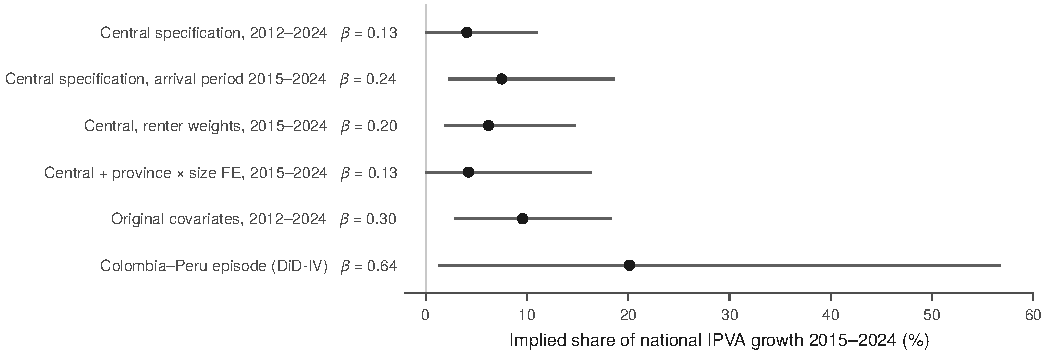
\includegraphics[width=0.85\linewidth]{fig/fig7_magnitude.pdf}
\caption{Implied contribution of immigration to national rent-index growth}\label{fig:magnitude}
\begin{minipage}{0.85\linewidth}\footnotesize\vspace{2pt}
\textit{Notes}: panel (a), implied share $\beta\times M/G$ under assumptions A1--A4. Panel (b), estimates and robust 95\,\% sets (analytical AR; wild-bootstrap AR for the episode).
\end{minipage}
\end{figure}

In relative terms, which require none of these assumptions, moving a municipality from the 10th to the 90th percentile of the annual inflow distribution (1.85 percentage points, table~\ref{tab:desc}) is associated with about $1.85\times\beta$ percentage points of additional annual growth of its rent index relative to its province: roughly 0.4 points with the central arrival-period estimate, against a difference of 5.7 points between the 10th and 90th percentiles of annual rent growth.

\section{Discussion}\label{sec:discussion}

\subsection{What the evidence supports}

The estimates support three statements. First, in the arrival years 2015--2024, municipalities receiving larger predicted inflows saw somewhat faster growth in the average rent of declared contracts in force than other municipalities in their province, of about \cenArrB\,\% per percentage point of inflow in the central specification (\cenArrAR), and larger in the Colombian-Peruvian episode. Second, there is no detectable response in the years of outflows. Third, the additional population was housed within the existing registered stock in the short run, with higher occupancy of primary dwellings and no detectable response of the cadastral stock.

\subsection{What is compatible with the evidence but not demonstrated}

Several interpretations are compatible with the results but not established by them: that pressure diffuses across the provincial or metropolitan market; that the national effect exceeds the local one; that entry rents respond more than the stock index; that conversion of vacant and second homes is the main supply margin; that natives relocate slowly; that higher occupancy reflects constraints rather than preferences; and that effects are larger for origins that rent more. Pre-specified heterogeneity by vacancy, density, rental depth and an effective rental-demand shock that weights origins by their housing consumption yields no interaction that survives a \citet{benjamini1995} correction (appendix table~\ref{tab:het}).

\subsection{What should not be inferred}

The data do not show that the main adjustment is overcrowding, that occupancy entails a cost borne by immigrants or by poorer households, that immigration explains a precise share of national rent growth, that rent caps shifted pressure to new contracts, or that the relevant scale for policy is the province because pressure spreads without a distance gradient. Earlier versions of this paper made some of these statements; they are not supported by the evidence presented here.

\subsection{Implications}

Two implications follow without overreaching. Price indices of contracts in force are incomplete indicators of demographic pressure: entry rents, room rents and occupancy relative to dwelling size should be measured regularly, and the Catalan deposit register shows that new-contract data at the municipal level are feasible. And because the occupied stock grew through more intensive use rather than construction, policies that expand the usable stock at the market level, by building or by bringing vacant dwellings into use, act on the margins through which newcomers are housed; this paper does not estimate the effect of such policies.

\section{Conclusions}\label{sec:conclusion}

Immigration after 2015 increased housing demand in Spain. In the short run, it was accommodated largely within the existing stock: registered population per dwelling rose with inflows, persons per primary dwelling rose between censuses, and the registered stock did not respond detectably. Within provinces, rents of declared contracts in force rose somewhat faster in municipalities receiving larger predicted inflows during the arrival years, by about \cenArrB\,\% per percentage point of inflow, an estimate smaller than in specifications with fewer controls, whose significance depends on assumptions about the origin shocks, and which a sharper visa-waiver episode suggests may be larger in large cities. The paper does not identify the effect of immigration on the national level of rents; under explicit assumptions, immigration accounts for a minority of the rise in the rent index. Higher occupancy is a quantitatively important margin that rent indices miss. Whether it reflects household structure, constraints or welfare losses requires data on rooms, entry rents and household composition at the local level that are not yet regularly available.

\section*{Statements and Declarations}

\noindent\textbf{Funding} The author did not receive support from any organization for the submitted work.

\medskip\noindent\textbf{Competing interests} The author has no relevant financial or non-financial interests to disclose.

\medskip\noindent\textbf{Ethics approval and consent} Not applicable. The study uses publicly available aggregate statistics and involves no human participants.

\medskip\noindent\textbf{Data availability} All data come from public sources: INE (IPVA; municipal register and annual population census by country of birth; 2011 and 2021 census tract indicators; central firm directory; statistics on migrations and changes of residence; household income atlas), the Directorate General for the Cadastre, the National Geographic Institute, Eurostat (EU-SILC, immigration by country of birth, local administrative units) and the Generalitat de Catalunya (Incasòl rental deposits, housing-policy areas). Analysis files and download scripts are in the replication package (Fernández-Aguilera 2026, \url{https://doi.org/10.5281/zenodo.23013308}, updated with the revision code).

\medskip\noindent\textbf{Code availability} The replication package contains the code that reproduces, from the official files, every number, table and figure in the paper.

\medskip\noindent\textbf{Use of generative AI} Claude (Anthropic) was used to retrieve the data, to write and run code and to draft and translate text. The author verified all results and text and is fully responsible for the article.

\medskip\noindent\textbf{Author contributions} The author is solely responsible for the conception, data collection, analysis and writing of the article.

\renewcommand{\refname}{References}
\begin{thebibliography}{99}\small\setlength{\itemsep}{2pt}\raggedright
\bibitem[Accetturo et~al.(2014)]{accetturo2014} Accetturo A, Manaresi F, Mocetti S, Olivieri E (2014) Don't stand so close to me: the urban impact of immigration. Regional Science and Urban Economics 45:45--56. \url{https://doi.org/10.1016/j.regsciurbeco.2014.01.001}
\bibitem[Adão et~al.(2019)]{adao2019} Adão R, Kolesár M, Morales E (2019) Shift-share designs: theory and inference. The Quarterly Journal of Economics 134(4):1949--2010. \url{https://doi.org/10.1093/qje/qjz025}
\bibitem[Akbari and Aydede(2012)]{akbari2012} Akbari AH, Aydede Y (2012) Effects of immigration on house prices in Canada. Applied Economics 44(13):1645--1658. \url{https://doi.org/10.1080/00036846.2010.548788}
\bibitem[Altonji and Card(1991)]{altonji1991} Altonji JG, Card D (1991) The effects of immigration on the labor market outcomes of less-skilled natives. In: Abowd JM, Freeman RB (eds) Immigration, trade, and the labor market. University of Chicago Press, Chicago, pp 201--234
\bibitem[Anderson and Rubin(1949)]{anderson1949} Anderson TW, Rubin H (1949) Estimation of the parameters of a single equation in a complete system of stochastic equations. The Annals of Mathematical Statistics 20(1):46--63. \url{https://doi.org/10.1214/aoms/1177730090}
\bibitem[Andrews et~al.(2019)]{andrews2019} Andrews I, Stock JH, Sun L (2019) Weak instruments in instrumental variables regression: theory and practice. Annual Review of Economics 11:727--753. \url{https://doi.org/10.1146/annurev-economics-080218-025643}
\bibitem[Balkan and Tumen(2016)]{balkan2016} Balkan B, Tumen S (2016) Immigration and prices: quasi-experimental evidence from Syrian refugees in Turkey. Journal of Population Economics 29(3):657--686. \url{https://doi.org/10.1007/s00148-016-0583-2}
\bibitem[Balkan et~al.(2018)]{balkan2018} Balkan B, Tok E, Torun H, Tumen S (2018) Immigration, housing rents, and residential segregation: evidence from Syrian refugees in Turkey. IZA Discussion Paper 11611, Institute of Labor Economics, Bonn
\bibitem[Banco de España(2024)]{bde2024} Banco de España (2024) El mercado de la vivienda en España: evolución reciente, riesgos y problemas de accesibilidad. In: Informe Anual 2023, chapter 4. Banco de España, Madrid
\bibitem[Benjamini and Hochberg(1995)]{benjamini1995} Benjamini Y, Hochberg Y (1995) Controlling the false discovery rate: a practical and powerful approach to multiple testing. Journal of the Royal Statistical Society: Series B 57(1):289--300.
\bibitem[Borusyak and Hull(2023)]{borusyak2023} Borusyak K, Hull P (2023) Nonrandom exposure to exogenous shocks. Econometrica 91(6):2155--2185. \url{https://doi.org/10.3982/ECTA19367}
\bibitem[Borusyak et~al.(2022)]{borusyak2022} Borusyak K, Hull P, Jaravel X (2022) Quasi-experimental shift-share research designs. The Review of Economic Studies 89(1):181--213. \url{https://doi.org/10.1093/restud/rdab030}
\bibitem[Borusyak et~al.(2025)]{borusyak2025} Borusyak K, Hull P, Jaravel X (2025) A practical guide to shift-share instruments. Journal of Economic Perspectives 39(1):181--204. \url{https://doi.org/10.1257/jep.20231370}
\bibitem[Card and DiNardo(2000)]{card2000} Card D, DiNardo J (2000) Do immigrant inflows lead to native outflows? American Economic Review 90(2):360--367. \url{https://doi.org/10.1257/aer.90.2.360}
\bibitem[Card(2001)]{card2001} Card D (2001) Immigrant inflows, native outflows, and the local labor market impacts of higher immigration. Journal of Labor Economics 19(1):22--64. \url{https://doi.org/10.1086/209979}
\bibitem[Chodorow-Reich(2020)]{chodorowreich2020} Chodorow-Reich G (2020) Regional data in macroeconomics: some advice for practitioners. Journal of Economic Dynamics and Control 115:103875.
\bibitem[Damm(2009)]{damm2009} Damm AP (2009) Determinants of recent immigrants' location choices: quasi-experimental evidence. Journal of Population Economics 22(1):145--174. \url{https://doi.org/10.1007/s00148-007-0148-5}
\bibitem[Davidson and MacKinnon(2010)]{davidson2010} Davidson R, MacKinnon JG (2010) Wild bootstrap tests for IV regression. Journal of Business \& Economic Statistics 28(1):128--144. \url{https://doi.org/10.1198/jbes.2009.07221}
\bibitem[Degen and Fischer(2017)]{degen2017} Degen K, Fischer AM (2017) Immigration and Swiss house prices. Swiss Journal of Economics and Statistics 153(1):15--36. \url{https://doi.org/10.1007/BF03399433}
\bibitem[Dustmann et~al.(2016)]{dustmann2016} Dustmann C, Schönberg U, Stuhler J (2016) The impact of immigration: why do studies reach such different results? Journal of Economic Perspectives 30(4):31--56. \url{https://doi.org/10.1257/jep.30.4.31}
\bibitem[Fernández-Aguilera(2026)]{fa2026} Fernández-Aguilera VM (2026) Replication package for: Immigration, rents and housing occupancy in Spain. Zenodo. \url{https://doi.org/10.5281/zenodo.23013308}
\bibitem[Fernández-Huertas Moraga et~al.(2019)]{fernandez2019} Fernández-Huertas Moraga J, Ferrer-i-Carbonell A, Saiz A (2019) Immigrant locations and native residential preferences: emerging ghettos or new communities? Journal of Urban Economics 112:133--151. \url{https://doi.org/10.1016/j.jue.2019.06.002}
\bibitem[Fieller(1954)]{fieller1954} Fieller EC (1954) Some problems in interval estimation. Journal of the Royal Statistical Society: Series B 16(2):175--185.
\bibitem[Garcia-López et~al.(2020)]{garcia2020} Garcia-López M-À, Jofre-Monseny J, Martínez-Mazza R, Segú M (2020) Do short-term rental platforms affect housing markets? Evidence from Airbnb in Barcelona. Journal of Urban Economics 119:103278. \url{https://doi.org/10.1016/j.jue.2020.103278}
\bibitem[Glaeser and Gyourko(2018)]{glaeser2018} Glaeser E, Gyourko J (2018) The economic implications of housing supply. Journal of Economic Perspectives 32(1):3--30. \url{https://doi.org/10.1257/jep.32.1.3}
\bibitem[Goldsmith-Pinkham et~al.(2020)]{goldsmith2020} Goldsmith-Pinkham P, Sorkin I, Swift H (2020) Bartik instruments: what, when, why, and how. American Economic Review 110(8):2586--2624. \url{https://doi.org/10.1257/aer.20181047}
\bibitem[Gonzalez and Ortega(2013)]{gonzalez2013} Gonzalez L, Ortega F (2013) Immigration and housing booms: evidence from Spain. Journal of Regional Science 53(1):37--59. \url{https://doi.org/10.1111/jors.12010}
\bibitem[Hanushek and Quigley(1980)]{hanushek1980} Hanushek EA, Quigley JM (1980) What is the price elasticity of housing demand? The Review of Economics and Statistics 62(3):449--454. \url{https://doi.org/10.2307/1927113}
\bibitem[Howard(2020)]{howard2020} Howard G (2020) The migration accelerator: labor mobility, housing, and demand. American Economic Journal: Macroeconomics 12(4):147--179. \url{https://doi.org/10.1257/mac.20180363}
\bibitem[Jaeger et~al.(2018)]{jaeger2018} Jaeger DA, Ruist J, Stuhler J (2018) Shift-share instruments and the impact of immigration. NBER Working Paper 24285, National Bureau of Economic Research, Cambridge, MA. \url{https://doi.org/10.3386/w24285}
\bibitem[Jordà(2005)]{jorda2005} Jordà Ò (2005) Estimation and inference of impulse responses by local projections. American Economic Review 95(1):161--182. \url{https://doi.org/10.1257/0002828053828518}
\bibitem[Khametshin et~al.(2024)]{khametshin2024} Khametshin D, López-Rodríguez D, Pérez García L (2024) El mercado del alquiler de vivienda residencial en España: evolución reciente, determinantes e indicadores de esfuerzo. Documentos Ocasionales 2432, Banco de España, Madrid
\bibitem[Lajer Baron et~al.(2024)]{lajer2024} Lajer Baron A, López Rodríguez D, San Juan L (2024) El mercado de la vivienda residencial en España: evolución reciente y comparación internacional. Documentos Ocasionales 2433, Banco de España, Madrid
\bibitem[Lee et~al.(2022)]{lee2022} Lee DS, McCrary J, Moreira MJ, Porter J (2022) Valid t-ratio inference for IV. American Economic Review 112(10):3260--3290.
\bibitem[López-Rodríguez and Matea(2019)]{lopez2019} López-Rodríguez D, Matea M de los Ll (2019) Evolución reciente del mercado del alquiler de vivienda en España. Boletín Económico 3/2019, Banco de España, Madrid
\bibitem[MacKinnon et~al.(2023)]{mackinnon2023} MacKinnon JG, Nielsen MØ, Webb MD (2023) Cluster-robust inference: a guide to empirical practice. Journal of Econometrics 232(2):272--299. \url{https://doi.org/10.1016/j.jeconom.2022.04.001}
\bibitem[Mocetti and Porello(2010)]{mocetti2010} Mocetti S, Porello C (2010) How does immigration affect native internal mobility? New evidence from Italy. Regional Science and Urban Economics 40(6):427--439. \url{https://doi.org/10.1016/j.regsciurbeco.2010.05.004}
\bibitem[Monràs and Garcia-Montalvo(2023)]{monras2023} Monràs J, Garcia-Montalvo J (2023) The effect of second-generation rent controls: new evidence from Catalonia. Working Paper 2023-28, Federal Reserve Bank of San Francisco. \url{https://doi.org/10.24148/wp2023-28}
\bibitem[Montiel Olea and Pflueger(2013)]{montiel2013} Montiel Olea JL, Pflueger C (2013) A robust test for weak instruments. Journal of Business \& Economic Statistics 31(3):358--369. \url{https://doi.org/10.1080/00401706.2013.806694}
\bibitem[Mussa et~al.(2017)]{mussa2017} Mussa A, Nwaogu UG, Pozo S (2017) Immigration and housing: a spatial econometric analysis. Journal of Housing Economics 35:13--25. \url{https://doi.org/10.1016/j.jhe.2017.01.002}
\bibitem[Myers and Lee(1996)]{myerslee1996} Myers D, Lee SW (1996) Immigration cohorts and residential overcrowding in southern California. Demography 33(1):51--65. \url{https://doi.org/10.2307/2061713}
\bibitem[Myers et~al.(1996)]{myers1996} Myers D, Baer WC, Choi S-Y (1996) The changing problem of overcrowded housing. Journal of the American Planning Association 62(1):66--84. \url{https://doi.org/10.1080/01944369608975671}
\bibitem[Ramey and Zubairy(2018)]{ramey2018} Ramey VA, Zubairy S (2018) Government spending multipliers in good times and in bad: evidence from US historical data. Journal of Political Economy 126(2):850--901. \url{https://doi.org/10.1086/696277}
\bibitem[Roback(1982)]{roback1982} Roback J (1982) Wages, rents, and the quality of life. Journal of Political Economy 90(6):1257--1278. \url{https://doi.org/10.1086/261120}
\bibitem[Roodman et~al.(2019)]{roodman2019} Roodman D, Nielsen MØ, MacKinnon JG, Webb MD (2019) Fast and wild: bootstrap inference in Stata using boottest. The Stata Journal 19(1):4--60. \url{https://doi.org/10.1177/1536867X19830877}
\bibitem[Sá(2015)]{sa2015} Sá F (2015) Immigration and house prices in the UK. The Economic Journal 125(587):1393--1424. \url{https://doi.org/10.1111/ecoj.12158}
\bibitem[Saiz and Wachter(2011)]{saiz2011} Saiz A, Wachter S (2011) Immigration and the neighborhood. American Economic Journal: Economic Policy 3(2):169--188. \url{https://doi.org/10.1257/pol.3.2.169}
\bibitem[Saiz(2003)]{saiz2003} Saiz A (2003) Room in the kitchen for the melting pot: immigration and rental prices. The Review of Economics and Statistics 85(3):502--521. \url{https://doi.org/10.1162/003465303322369687}
\bibitem[Saiz(2007)]{saiz2007} Saiz A (2007) Immigration and housing rents in American cities. Journal of Urban Economics 61(2):345--371. \url{https://doi.org/10.1016/j.jue.2006.07.004}
\bibitem[Saiz(2010)]{saiz2010} Saiz A (2010) The geographic determinants of housing supply. The Quarterly Journal of Economics 125(3):1253--1296. \url{https://doi.org/10.1162/qjec.2010.125.3.1253}
\bibitem[Sanchis-Guarner(2023)]{sanchis2023} Sanchis-Guarner R (2023) Decomposing the impact of immigration on house prices. Regional Science and Urban Economics 100:103893. \url{https://doi.org/10.1016/j.regsciurbeco.2023.103893}
\bibitem[Sanderson and Windmeijer(2016)]{sanderson2016} Sanderson E, Windmeijer F (2016) A weak instrument F-test in linear IV models with multiple endogenous variables. Journal of Econometrics 190(2):212--221.
\bibitem[Solon et~al.(2015)]{solon2015} Solon G, Haider SJ, Wooldridge JM (2015) What are we weighting for? Journal of Human Resources 50(2):301--316.
\bibitem[Tumen(2016)]{tumen2016} Tumen S (2016) The economic impact of Syrian refugees on host countries: quasi-experimental evidence from Turkey. American Economic Review 106(5):456--460. \url{https://doi.org/10.1257/aer.p20161065}
\bibitem[Unal et~al.(2026)]{unal2026} Unal U, Hayo B, Erol I (2026) The effect of immigration on housing prices: evidence from 382 German districts. The Journal of Real Estate Finance and Economics 72(2):386--424. \url{https://doi.org/10.1007/s11146-024-09988-x}
\bibitem[Webb(2023)]{webb2023} Webb MD (2023) Reworking wild bootstrap-based inference for clustered errors. Canadian Journal of Economics 56(3):839--858. \url{https://doi.org/10.1111/caje.12661}
\bibitem[Wolf(2023)]{wolf2023} Wolf CK (2023) The missing intercept: a demand equivalence approach. American Economic Review 113(8):2232--2269.
\end{thebibliography}


\clearpage
\appendix
\section*{Appendix A. Data construction and sources}
\addcontentsline{toc}{section}{Appendix A}

\textit{Rents.} INE IPVA, tables 59060 (municipalities), 59061 (districts), 59058, 59059 and 59005 (provinces). The general index (base 2015) and its annual log difference are used. Catalan new contracts: Generalitat de Catalunya open data, ``Preu mitjà del lloguer d'habitatges per municipi'' (Incasòl deposit register), annual January--December mean rent and number of contracts.

\textit{Population.} INE municipal register by country of birth (table 33573), 2003--2022, and annual population census (table 66322), 2021--2025, downloaded from INE and harmonised into 33 groups (28 countries and five continental residuals). Municipalities created after 2003 receive zero shares. Flows in year $t$ are the difference between 1 January of $t+1$ and of $t$ within the same source: register up to $t=2021$ and annual census from $t=2022$. The rebuilt instrument reproduces the one used in the earlier version of the paper exactly. Intermunicipal migration of the Spain-born: INE statistics on migrations and changes of residence, tables 69744 and 69746 (2021--2024).

\textit{Censuses.} Tract-level indicators for 2011 (INE, indicators by census tract: population by region of birth, education, age, tenure, rooms and floor area of primary dwellings, households) and 2021 (population, foreign-born, dwellings, tenure, households), aggregated to municipalities. Suppressed tract cells are imputed with the municipal ratio of the variable to population.

\textit{Firm directory and geography.} INE central firm directory (DIRCE), table 4721, firms by municipality and activity in 2012. Eurostat correspondence of local administrative units (LAU 2021): degree of urbanisation, coastal flag, city and functional urban area. IGN boundary lines for distances and contiguity, as in the earlier version.

\textit{Cadastre and other.} Directorate General for the Cadastre, dwellings by district, aggregated to municipalities (2015--2025). INE household income atlas (2015) and experimental tourist dwellings. Generalitat de Catalunya, housing-policy areas (tensioned residential market zones and areas of strong demand). Eurostat: EU-SILC (ilc\_lvho15, ilc\_lvps15) and immigration by country of birth (migr\_imm3ctb).

\textit{Sources that could not be used.} The Ministry of Housing's appraisal values (which would provide pre-2011 price trends), the bulk files of the State Reference System of Rental Prices (SERPAVI) and the Atlas of Urban Areas could not be downloaded from the environment in which the revision was produced; the Eurostat FUA delimitation is used instead of the latter. The municipal register by nationality for 1998--2002 is available from INE only at national and provincial level, so older municipal shares could not be built. Municipal births by mother's nationality and municipal registered unemployment were not obtained. These limitations are discussed in section~\ref{sec:discussion}.

\textit{Replication.} The revision code rebuilds the instrument from the INE downloads and produces every number, table and figure; numbers in the text are read from the results. Estimates use \texttt{pyfixest} and \texttt{linearmodels} in Python; residualisation, Anderson-Rubin sets, the wild bootstrap, randomisation inference, AKM0 and Fieller intervals are coded explicitly.

\clearpage
\section*{Appendix B. Model derivations}
\addcontentsline{toc}{section}{Appendix B}

\textit{Local equilibrium.} Housing demand is $H_i^d=(a_NN_i+a_MM_i)R_i^{-\eta}$. Log-differentiating,
\[
\hat H_i^d=\frac{a_N\,dN_i+a_M\,dM_i}{a_NN_i+a_MM_i}-\eta\hat R_i=(1-\theta_i)\hat N_i+\kappa\,m_i-\eta\hat R_i,
\]
where $1-\theta_i=a_NN_i/(a_NN_i+a_MM_i)$, $m_i=dM_i/P_i$ and $\kappa=a_M/\bar a$. Native mobility gives $\hat N_i=-\delta(\hat R_i-\hat R_j)$ and supply $\hat H_i^s=\varepsilon\hat R_i$. Equating yields \eqref{eq:eq} with $\delta'=(1-\theta)\delta$.

\textit{Proposition~\ref{prop:scale}.} Adding cross-market mobility with elasticity $\delta_J$ and averaging over the market's locations, $(\varepsilon+\eta+\delta'_J)\hat R_j=\kappa\bar m$, so $\beta_J=\kappa/(\varepsilon+\eta+\delta'_J)$. Subtracting the market equation from the local one, $\kappa(m_i-\bar m)=(\varepsilon+\eta+\delta')(\hat R_i-\hat R_j)$, so $\beta_L=\kappa/(\varepsilon+\eta+\delta')$.

\textit{Absorption accounting.} In deviations from the market, $\hat R_i=\beta_Lm_i$, $\hat H_i=\varepsilon\beta_Lm_i$ and, if natives consume the average dwelling, the change in natives per inhabitant is $n_i=-\delta'\beta_Lm_i$. Population grows by $\hat P_i=m_i+n_i$ and occupancy by $\hat s_i=\hat P_i-\hat H_i$, so $c=\hat s_i/m_i=1-(\varepsilon+\delta')\beta_L$ and, since $(\varepsilon+\eta+\delta')\beta_L=\kappa$, $c=1-\kappa+\eta\beta_L$. The earlier version of the paper inverted these relations to obtain $\varepsilon+\delta'=(1-c)/\beta_L$. With the robust sets for $\beta_L$ reported in table~\ref{tab:main}, which include values close to zero, this ratio is not bounded above, and the paper does not report point values for $\varepsilon$ or $\delta'$. With $\beta_L$ small, the model attributes most of $c$ to composition, $1-\kappa$; section~\ref{sec:margins} shows that composition across continental groups does not account for the observed change, which in the model requires either newcomers with much lower $\kappa$ than settled immigrants of the same origin or a larger price term.

\textit{Relation to the census decomposition.} Identity \eqref{eq:identity} is the discrete version of $\hat P_i=\hat H_i+\hat s_i$, with the occupied stock split into total stock and non-primary dwellings.

\clearpage
\section*{Appendix C. Additional tables and figures}
\addcontentsline{toc}{section}{Appendix C}
\begin{table}[!htbp]\centering\small
\caption{Sample flow}\label{tab:flow}
\begin{tabular}{lr}\toprule
Municipalities in the Padrón (2003--2022) & 8,136\\
Municipalities with an IPVA (INE table 59060) & 718\\
Municipality-years with IPVA growth, 2012--2024 & 9,138\\
Analysis sample after dropping singleton province-years and missing covariates & 9,060 (699 municipalities, 42 provinces)\\
Census long-difference sample (municipalities above 5,000 inhabitants) & 1,265\\
\bottomrule\end{tabular}
\begin{minipage}{0.9\linewidth}\footnotesize\vspace{4pt}\textit{Notes}: the IPVA excludes the Basque Country and Navarre. Province-years with a single sample municipality are dropped because the province $\times$ year fixed effect absorbs them.\end{minipage}\end{table}
\begin{table}[!htbp]\centering\small
\caption{Estimates and inference with renter weights}\label{tab:main_rent}
\begin{adjustbox}{max width=\linewidth}\begin{tabular}{lcccc}\toprule
 & (1) Minimal & (2) Original & (3) Central & (4) Central + size FE \\ \midrule
\multicolumn{5}{l}{\textit{A. Full period, 2012--2024}}\\
OLS & 0.15 & 0.07 & 0.07 & 0.05 \\
Reduced form & 0.28 & 0.11 & 0.06 & 0.01 \\
First-stage $F$ & 28.7 & 36.4 & 36.2 & 41.1 \\
2SLS & 0.50 & 0.30 & 0.14 & 0.03 \\
 & (0.12) & (0.10) & (0.09) & (0.11) \\
AR 95\% set, province clusters & [0.31, 0.84] & [0.12, 0.54] & [$-$0.02, 0.33] & [$-$0.19, 0.27] \\
AR 95\% set, wild bootstrap & [0.24, 0.88] & [0.07, 0.54] & [$-$0.07, 0.34] & [$-$0.23, 0.31] \\
Randomisation, all origins & [0.35, 0.74] & [0.20, 0.43] & [0.07, 0.23] & [$-$0.06, 0.19] \\
Randomisation, size terciles & [0.24, 0.77] & [0.15, 0.41] & [0.02, 0.29] & [$-$0.14, 0.24] \\
Randomisation, within continents & [$-$0.45, 1.70] & $(-\infty,\infty)$ & $(-\infty,\infty)$ & $(-\infty,\infty)$ \\
2SLS with national shocks & 0.47 & 0.26 & 0.13 & 0.03 \\
AKM0 95\% set, shocks clustered by origin & [0.30, 0.99] & [$-$0.02, 0.76] & [$-$0.65, 0.38] & [$-$0.75, 0.44] \\
Observations & 9,060 & 9,060 & 9,060 & 8,449 \\
\midrule
\multicolumn{5}{l}{\textit{B. Arrival period, 2015--2024}}\\
OLS & 0.20 & 0.11 & 0.10 & 0.08 \\
Reduced form & 0.27 & 0.12 & 0.08 & 0.04 \\
First-stage $F$ & 21.3 & 15.1 & 17.3 & 19.8 \\
2SLS & 0.51 & 0.39 & 0.20 & 0.12 \\
 & (0.11) & (0.14) & (0.09) & (0.11) \\
AR 95\% set, province clusters & [0.34, 0.84] & [0.17, 0.83] & [0.06, 0.47] & [$-$0.07, 0.43] \\
AR 95\% set, wild bootstrap & [0.30, 1.13] & [0.14, 0.87] & [0.03, 0.49] & [$-$0.08, 0.47] \\
Randomisation, all origins & [0.40, 0.68] & [0.27, 0.55] & [0.14, 0.26] & [0.06, 0.23] \\
Randomisation, size terciles & [0.32, 0.63] & [0.22, 0.51] & [0.11, 0.31] & [$-$0.01, 0.25] \\
Randomisation, within continents & [$-$0.06, 0.89] & $(-\infty,\infty)$ & $(-\infty,\infty)$ & $(-\infty,\infty)$ \\
2SLS with national shocks & 0.49 & 0.34 & 0.18 & 0.12 \\
AKM0 95\% set, shocks clustered by origin & [0.32, 3.80] & [0.04, $\infty$] & [$-$0.94, 0.48] & [$-$0.87, 0.48] \\
Observations & 6,972 & 6,972 & 6,972 & 6,502 \\
\bottomrule
\end{tabular}\end{adjustbox}
\begin{minipage}{0.97\linewidth}\footnotesize\vspace{4pt}
\textit{Notes}: dependent variable $\Delta\ln R_{it}$, annual growth of the municipal IPVA; treatment $m_{it}$, foreign-born inflow over population (centred timing); instrument $z_{it}$, 2003 shares of 33 origins times national growth excluding the own province. All columns include province $\times$ year fixed effects and the 2003 foreign-born share interacted with every year. Column 2 adds the original covariates (log income per person 2015, log population 2011, 2011 shares of renting households and non-primary dwellings) $\times$ year; column 3 replaces them with the central set of predetermined covariates (2011 census: log population, renting share, non-primary share, tertiary-education share, share aged 65+; 2012 firm directory: shares of construction, industry and trade-transport-hospitality firms and firms per capita; coastal and FUA-core indicators) $\times$ year; column 4 adds province $\times$ size class $\times$ year fixed effects. Anderson-Rubin (AR) sets invert the reduced-form test with province-clustered errors (analytical) or with 4,999 restricted wild-bootstrap draws with Webb weights. Randomisation sets permute the growth paths of origins 2,000 times within the indicated strata, recentre the instrument and invert the studentised reduced-form test. The last two rows use national (not leave-out) shocks; AKM0 is the null-imposed exposure-robust test of \citet{adao2019} with origin-year shocks clustered by origin. $\infty$ denotes an unbounded set. Weights: rented main dwellings, 2011 census.
\end{minipage}\end{table}
\begin{table}[!htbp]\centering\small
\caption{Estimates and inference, unweighted}\label{tab:main_unw}
\begin{adjustbox}{max width=\linewidth}\begin{tabular}{lcccc}\toprule
 & (1) Minimal & (2) Original & (3) Central & (4) Central + size FE \\ \midrule
\multicolumn{5}{l}{\textit{A. Full period, 2012--2024}}\\
OLS & 0.08 & 0.07 & 0.08 & 0.07 \\
Reduced form & 0.11 & 0.06 & 0.00 & $-$0.01 \\
First-stage $F$ & 12.0 & 14.5 & 15.7 & 13.6 \\
2SLS & 0.35 & 0.21 & 0.01 & $-$0.02 \\
 & (0.15) & (0.15) & (0.16) & (0.19) \\
AR 95\% set, province clusters & [0.08, 0.83] & [$-$0.11, 0.57] & [$-$0.37, 0.34] & [$-$0.48, 0.39] \\
AR 95\% set, wild bootstrap & [0.05, 0.86] & [$-$0.18, 0.60] & [$-$0.42, 0.37] & [$-$0.54, 0.41] \\
Randomisation, all origins & [0.13, 0.92] & [0.02, 0.60] & [$-$0.16, 0.38] & [$-$0.20, 0.42] \\
Randomisation, size terciles & [$-$0.03, 0.88] & [$-$0.11, 0.53] & [$-$0.25, 0.41] & [$-$0.29, 0.49] \\
Randomisation, within continents & $(-\infty,\infty)$ & $(-\infty,\infty)$ & $(-\infty,\infty)$ & $(-\infty,\infty)$ \\
2SLS with national shocks & 0.29 & 0.16 & 0.03 & 0.01 \\
AKM0 95\% set, shocks clustered by origin & [$-$0.18, 1.33] & [$-$0.63, 1.03] & [$-$1.26, 0.75] & [$-$1.25, 0.92] \\
Observations & 9,060 & 9,060 & 9,060 & 8,449 \\
\midrule
\multicolumn{5}{l}{\textit{B. Arrival period, 2015--2024}}\\
OLS & 0.15 & 0.15 & 0.14 & 0.13 \\
Reduced form & 0.16 & 0.10 & 0.04 & 0.04 \\
First-stage $F$ & 5.2 & 5.3 & 6.1 & 6.1 \\
2SLS & 0.66 & 0.57 & 0.19 & 0.19 \\
 & (0.28) & (0.30) & (0.20) & (0.25) \\
AR 95\% set, province clusters & [0.32, $\infty$] & [0.17, 3.65] & [$-$0.15, 1.41] & [$-$0.24, 1.70] \\
AR 95\% set, wild bootstrap & [0.31, 3.74] & [0.14, 3.51] & [$-$0.15, 1.43] & [$-$0.23, 1.48] \\
Randomisation, all origins & [0.48, 1.80] & [0.41, 1.31] & [0.07, 0.60] & [0.05, 0.73] \\
Randomisation, size terciles & [0.44, 2.38] & [0.36, 1.30] & [$-$0.03, 0.66] & [$-$0.04, 0.82] \\
Randomisation, within continents & [0.16, 0.72] & [$-$0.82, 0.77] & $(-\infty,\infty)$ & [$-$0.97, 0.91] \\
2SLS with national shocks & 0.62 & 0.53 & 0.21 & 0.22 \\
AKM0 95\% set, shocks clustered by origin & [0.20, $\infty$] & $(-\infty,\infty)$ & $(-\infty,\infty)$ & $(-\infty,\infty)$ \\
Observations & 6,972 & 6,972 & 6,972 & 6,502 \\
\bottomrule
\end{tabular}\end{adjustbox}
\begin{minipage}{0.97\linewidth}\footnotesize\vspace{4pt}
\textit{Notes}: dependent variable $\Delta\ln R_{it}$, annual growth of the municipal IPVA; treatment $m_{it}$, foreign-born inflow over population (centred timing); instrument $z_{it}$, 2003 shares of 33 origins times national growth excluding the own province. All columns include province $\times$ year fixed effects and the 2003 foreign-born share interacted with every year. Column 2 adds the original covariates (log income per person 2015, log population 2011, 2011 shares of renting households and non-primary dwellings) $\times$ year; column 3 replaces them with the central set of predetermined covariates (2011 census: log population, renting share, non-primary share, tertiary-education share, share aged 65+; 2012 firm directory: shares of construction, industry and trade-transport-hospitality firms and firms per capita; coastal and FUA-core indicators) $\times$ year; column 4 adds province $\times$ size class $\times$ year fixed effects. Anderson-Rubin (AR) sets invert the reduced-form test with province-clustered errors (analytical) or with 4,999 restricted wild-bootstrap draws with Webb weights. Randomisation sets permute the growth paths of origins 2,000 times within the indicated strata, recentre the instrument and invert the studentised reduced-form test. The last two rows use national (not leave-out) shocks; AKM0 is the null-imposed exposure-robust test of \citet{adao2019} with origin-year shocks clustered by origin. $\infty$ denotes an unbounded set. Unweighted.
\end{minipage}\end{table}
\begin{table}[!htbp]\centering\small
\caption{Leave-one-out estimates (central specification, population weights, 2012--2024)}\label{tab:loo}
\begin{tabular}{lcccc}\toprule
Excluded unit & Number & Min & Median & Max\\\midrule
One province & 42 & 0.03 & 0.13 & 0.18\\
One autonomous community & 15 & 0.03 & 0.13 & 0.19\\
One origin from the instrument & 33 & 0.05 & 0.13 & 0.23\\
One continent from the instrument & 4 & 0.08 & 0.17 & 0.48\\
\bottomrule\end{tabular}
\end{table}
\begin{table}[!htbp]\centering\scriptsize
\caption{Rotemberg decomposition by origin (original specification, population weights)}\label{tab:rotfull}
\begin{tabular}{llrrrrr}\toprule
Origin & Continent & $\hat\alpha_o$ & $\hat\beta_o$ & $F_o$ & $\hat\alpha_o\hat\beta_o$ & $g_{2012-24}$\\\midrule
Romania & Europe & 0.314 & 0.39 & 27.0 & 0.124 & $-$2.33\\
Colombia & Americas & 0.210 & 0.68 & 14.9 & 0.143 & 2.34\\
United Kingdom & Europe & 0.140 & $-$0.52 & 6.1 & $-$0.072 & $-$0.66\\
Peru & Americas & 0.103 & $-$0.05 & 60.1 & $-$0.005 & 3.20\\
Germany & Europe & 0.100 & $-$0.54 & 12.1 & $-$0.054 & $-$0.38\\
Ukraine & Europe & 0.051 & $-$0.24 & 0.8 & $-$0.012 & 2.98\\
Venezuela & Americas & 0.047 & 1.55 & 2.1 & 0.072 & 6.35\\
Russia & Europe & 0.044 & $-$0.02 & 5.6 & $-$0.001 & 2.50\\
Rest of Americas & Americas & 0.036 & 0.42 & 3.1 & 0.015 & 4.73\\
Cuba & Americas & 0.026 & 0.52 & 3.6 & 0.014 & 2.01\\
Dominican Republic & Americas & 0.019 & 0.51 & 5.2 & 0.009 & 1.02\\
Bulgaria & Europe & 0.018 & 0.67 & 6.5 & 0.012 & $-$1.30\\
Pakistan & Asia & 0.014 & 0.94 & 0.6 & 0.013 & 2.75\\
Rest of Asia & Asia & 0.010 & $-$0.54 & 0.1 & $-$0.005 & 1.87\\
Bolivia & Americas & 0.010 & $-$1.16 & 5.4 & $-$0.011 & 0.02\\
Poland & Europe & 0.009 & 1.54 & 4.2 & 0.013 & $-$0.95\\
China & Asia & 0.006 & 0.64 & 0.8 & 0.004 & 0.99\\
Algeria & Africa & 0.005 & $-$0.31 & 1.0 & $-$0.001 & 0.93\\
Ecuador & Americas & 0.005 & $-$1.21 & 0.1 & $-$0.005 & $-$0.00\\
Chile & Americas & 0.001 & $-$3.94 & 0.0 & $-$0.003 & 0.47\\
Brazil & Americas & 0.000 & 11.46 & 0.0 & 0.005 & 1.25\\
Nigeria & Africa & 0.000 & 13.11 & 0.0 & 0.002 & $-$0.13\\
Oceania and other & Other & $-$0.000 & $-$13.25 & 0.0 & 0.000 & 0.62\\
Rest of Africa & Africa & $-$0.001 & $-$19.91 & 0.0 & 0.022 & 0.90\\
Portugal & Europe & $-$0.002 & 4.91 & 0.1 & $-$0.010 & $-$0.67\\
Senegal & Africa & $-$0.002 & $-$8.09 & 0.0 & 0.019 & 2.76\\
Italy & Europe & $-$0.006 & $-$3.61 & 0.2 & 0.021 & 1.51\\
Argentina & Americas & $-$0.007 & $-$5.30 & 0.1 & 0.035 & 0.89\\
Uruguay & Americas & $-$0.007 & 0.22 & 3.2 & $-$0.002 & 0.20\\
France & Europe & $-$0.009 & 1.08 & 6.2 & $-$0.010 & $-$0.02\\
Paraguay & Americas & $-$0.016 & 0.10 & 9.8 & $-$0.002 & 19.95\\
Morocco & Africa & $-$0.039 & $-$0.73 & 0.5 & 0.029 & 0.94\\
Rest of Europe & Europe & $-$0.077 & 0.74 & 10.6 & $-$0.057 & 0.20\\
\bottomrule\end{tabular}
\end{table}
\begin{table}[!htbp]\centering\small
\caption{Pre-specified heterogeneity (central specification)}\label{tab:het}
\begin{tabular}{lcccc}\toprule
Dimension & Weights & Interaction (s.e.) & $p$ & BH $q$\\\midrule
H1a vacancy 2011 & w & $-$0.02 (0.02) & 0.371 & 0.59\\
H1a vacancy 2011 & unw & $-$0.02 (0.05) & 0.748 & 0.75\\
H1b log density 2011 & w & $-$0.03 (0.04) & 0.569 & 0.69\\
H1b log density 2011 & unw & $-$0.03 (0.06) & 0.602 & 0.69\\
H2 renting share 2011 & w & $-$0.07 (0.04) & 0.107 & 0.29\\
H2 renting share 2011 & unw & $-$0.11 (0.05) & 0.046 & 0.18\\
H3 effective-demand horse race (reduced form) & w & $-$0.24 (0.21) & 0.275 & 0.55\\
H3 effective-demand horse race (reduced form) & unw & $-$0.46 (0.20) & 0.027 & 0.18\\
\bottomrule\end{tabular}
\begin{minipage}{0.95\linewidth}\footnotesize\vspace{4pt}\textit{Notes}: H1 and H2: 2SLS with the inflow and its interaction with the standardised characteristic, instrumented with the instrument and its interaction; the characteristic $\times$ year is controlled for. H3: reduced form with the instrument and an effective rental-demand instrument that weights each origin by its relative housing consumption $\kappa$ (table~\ref{tab:kappa}); the coefficient reported is that of the effective-demand instrument. $q$: Benjamini-Hochberg adjusted over the eight tests.\end{minipage}\end{table}
\begin{table}[!htbp]\centering\small
\caption{Stock index and new-contract rents in Catalonia (Incasòl deposit register)}\label{tab:catalonia}
\begin{adjustbox}{max width=\linewidth}\begin{tabular}{lc}\toprule
Municipalities matched to the analysis sample & 123\\
Median annual new contracts per rented main dwelling (2011 census) & 0.31\\
Correlation of annual growth: IPVA vs mean new-contract rent & 0.59\\
IPVA growth on new-contract rent growth, contemporaneous (municipality and year FE) & 0.028 (0.005)\\
\quad with two lags: $t$ / $t-1$ / $t-2$ & 0.034 / 0.039 / 0.036\\
2SLS within Catalonia, central covariates: first-stage $F$ & 4.2\\
\quad IPVA / new-contract rent / log contracts per capita & $-$0.07 / $-$0.19 / $-$4.15\\
\bottomrule\end{tabular}\end{adjustbox}
\begin{minipage}{0.95\linewidth}\footnotesize\vspace{4pt}\textit{Notes}: annual (January--December) mean monthly rent and number of new contracts with a deposit lodged at Incasòl, by municipality (Generalitat de Catalunya open data). Within-Catalonia 2SLS uses municipality clusters because only four provinces are available; the instrument is weak in this subsample and the estimates are reported for completeness.\end{minipage}\end{table}
\begin{table}[!htbp]\centering\small
\caption{Alternative push shocks and spatial spillovers (central specification)}\label{tab:altspatial}
\begin{tabular}{lcc}\toprule
 & Population weights & Unweighted\\\midrule
\multicolumn{3}{l}{\textit{A. Shifts from inflows of each origin into 12 other European countries (Eurostat)}}\\
First-stage $F$ & 0.11 & 0.12\\
2SLS (AR set) & 0.97 $(-\infty,\infty)$ & 1.78 $(-\infty,\infty)$\\
\midrule\multicolumn{3}{l}{\textit{B. Own inflow and inflow into the surroundings (both instrumented)}}\\
Contiguous municipalities: own & 0.13 (0.11) & $-$0.00 (0.16)\\
\quad surroundings & 0.06 (0.07) & 0.03 (0.07)\\
Ring 0--15 km: own & 0.14 (0.10) & 0.02 (0.15)\\
\quad surroundings & 0.01 (0.10) & 0.09 (0.07)\\
Ring 15--40 km: own & 0.13 (0.11) & 0.02 (0.17)\\
\quad surroundings & $-$0.05 (0.10) & $-$0.09 (0.14)\\
\bottomrule\end{tabular}
\begin{minipage}{0.95\linewidth}\footnotesize\vspace{4pt}\textit{Notes}: panel A: destinations AT, BG, CZ, FI, HR, IT, LU, NL, NO, SE, SI and SK (Eurostat migr\_imm3ctb, isolated gaps interpolated); the shift is the inflow of each of the 28 individual origins into these countries over its 2003 stock in Spain. Panel B: surroundings defined as in the original manuscript (all municipalities, with or without an IPVA).\end{minipage}\end{table}
\begin{table}[!htbp]\centering\small
\caption{Relative housing consumption by region of birth, 2011 census tracts}\label{tab:kappa}
\begin{tabular}{lcc}\toprule
Region of birth & Dwellings per person & $\kappa$ (relative to the average resident)\\\midrule
Spain & 0.386 & 1.01\\
Europe & 0.421 & 1.10\\
Africa & 0.244 & 0.64\\
America & 0.368 & 0.96\\
Asia & 0.261 & 0.68\\
Oceania & 0.614 & 1.60\\
\bottomrule\end{tabular}
\begin{minipage}{0.9\linewidth}\footnotesize\vspace{4pt}\textit{Notes}: ecological regression of primary dwellings per person on population shares by region of birth across 24,030 census tracts with at least 100 inhabitants, with municipality fixed effects and population weights.\end{minipage}\end{table}

\begin{figure}[!htbp]\centering
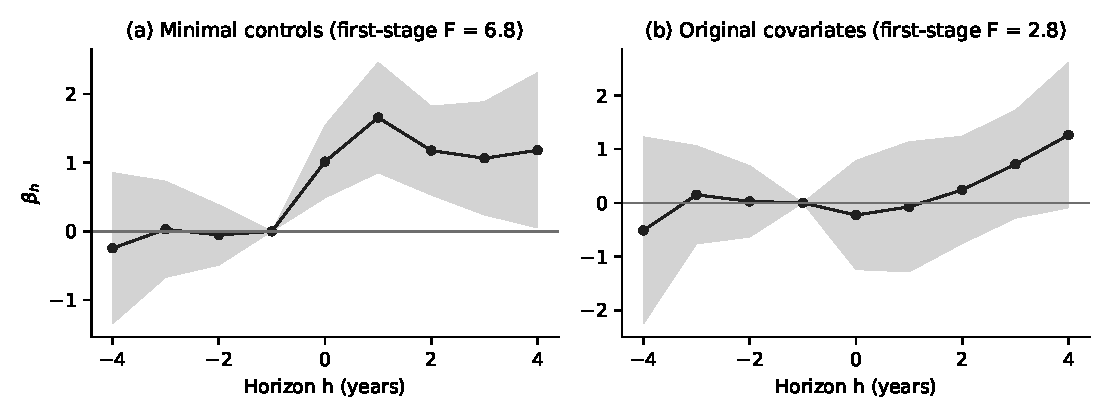
\includegraphics[width=\linewidth]{fig/figA1_lp.pdf}
\caption{Local projections identified from innovations in the instrument}\label{fig:lp}
\begin{minipage}{0.95\linewidth}\footnotesize\vspace{2pt}
\textit{Notes}: coefficients $\beta_h$ of $\ln R_{i,t+h}-\ln R_{i,t-1}$ on the calendar-year inflow instrumented with its prediction, controlling for three lags of the prediction, province $\times$ year fixed effects and the indicated controls; balanced sample $t\in[2015,2020]$; population weights; 95\,\% intervals with province clusters. The first-stage $F$ in the title shows that innovations in the instrument carry little predictive power.
\end{minipage}
\end{figure}

\end{document}
